\documentclass[12pt,a4paper,twoside,openright]{book}
\usepackage[utf8]{inputenc}
\usepackage[spanish,es-tabla]{babel}
\usepackage{graphicx}
\usepackage{amssymb}
\usepackage{amsmath}
\usepackage{hyperref}
\usepackage{enumitem}
\usepackage{fancyhdr}
\usepackage{datetime2}
\usepackage{multicol}
\usepackage[round,authoryear,sort]{natbib}
\usepackage{doi} % show dois as links on references
\usepackage{mathpazo} % Use the Palatino font by default

% Change margins at each side of the page
\addtolength{\oddsidemargin}{1cm}
\addtolength{\evensidemargin}{-1cm}

% Import variables
% Title, authors and affiliations
\newcommand{\Title}{TITLE}
\newcommand{\Soler}{Santiago Rubén Soler}
\newcommand{\SolerShort}{S.R. Soler}
\newcommand{\SolerMail}{santiago.r.soler@gmail.com}
\newcommand{\CONICET}{%
    CONICET, Argentina
}
\newcommand{\IGSV}{%
    Instituto Geofísico Sismológico Volponi, Universidad Nacional de San Juan, Argentina
}

% DOIs
\newcommand{\ThesisDOI}{XX.XXXXX/XXXXXX}

% Define inverse symbol with shorter minus
\newcommand{\inv}{^{\text{-}1}}
\newcommand{\trans}{^{\text{T}}}

% Define some units
\newcommand{\m}{$\,$m}
\newcommand{\km}{$\,$km}
\newcommand{\mGal}{$\,$mGal}



% Configure hyperref and add PDF metadata
\hypersetup{
    colorlinks,
    allcolors=[rgb]{0, 0.451, 0.753},
    pdftitle={\Title},
    pdfauthor={\Soler},
    pdfsubject={\PDFSubject},
    pdfkeywords={\PDFKeywords},
    pdftex,
}
\urlstyle{same}


% Configure headers and footers
% -----------------------------
% Configure every page of the thesis with a fancy style
\pagestyle{fancy}

% Define a command for configuring headers and footers of frontmatter
\newcommand{\fancyfront}{%
    \fancyhf{} % clear all header and footer fields
    \fancyfoot[C]{\thepage}
    \renewcommand{\headrulewidth}{0pt}
    \renewcommand{\footrulewidth}{0pt}

    % Override headers and footers for chapter pages
    \fancypagestyle{plain}{%
        \fancyhf{} % clear all header and footer fields
        \fancyfoot[C]{\thepage}
        \renewcommand{\headrulewidth}{0pt}
        \renewcommand{\footrulewidth}{0pt}
    }
}

% Define a command for configuring headers and footers of mainmatter
\newcommand{\fancymain}{%
    \fancyhf{} % clear all header and footer fields
    \fancyhead[RO,LE]{\thepage}
    \fancyhead[RE]{\leftmark}
    \fancyhead[LO]{\nouppercase{\rightmark}}
    \renewcommand{\headrulewidth}{0.4pt}

    % Override headers and footers for chapter pages
    \fancypagestyle{plain}{%
        \fancyhf{} % clear all header and footer fields
        \renewcommand{\headrulewidth}{0pt}
        \renewcommand{\footrulewidth}{0pt}
    }

}

% Clear headers and footers on blank pages before new chapter
\makeatletter
\def\cleardoublepage{
    \clearpage
    \if@twoside
        \ifodd\c@page
        \else\hbox{}\thispagestyle{empty}\newpage
            \if@twocolumn\hbox{}\newpage
            \fi
        \fi
    \fi
}
\makeatother

% Source: https://tug.org/pracjourn/2008-1/mori/mori.pdf


% =============================================================================

\begin{document}

\frontmatter
\fancyfront

\begin{titlepage}

    \begin{center}

        
\includegraphics[height=4cm]{figs/logos/unsj.pdf}
        \vspace{1.5em}

        {\Large
        UNIVERSIDAD NACIONAL DE SAN JUAN \\
        FACULTAD DE CIENCIAS EXACTAS, FÍSICAS Y NATURALES \\
        INSTITUTO GEOFÍSICO SISMOLÓGICO VOLPONI \\
        }
        \vspace{3em}

        \textbf{\huge TESIS DOCTORAL}
        \vspace{3em}

        \textbf{\Huge \Title}

        \vspace{\fill}

        \textbf{\LARGE Autor}
        \vspace{1em}

        {\LARGE \LicSoler{}}
        \vspace{1.5em}

        \rule{\linewidth}{1px}
        \vspace{1.5em}

        \begin{minipage}{0.45\linewidth}
            \raggedright
            \textbf{\LARGE Director}
            \vspace{1em}

            {\LARGE \Mario{}}
        \end{minipage}
        \begin{minipage}{0.45\linewidth}
            \raggedleft
            \textbf{\LARGE Codirector}
            \vspace{1em}

            {\LARGE \Leo{}}
        \end{minipage}

    \end{center}

\end{titlepage}


\vspace*{\fill}
%
\textit{\Title{}} \\
por \Soler{}

\ifthenelse{\equal{\ThesisDOI}{}}{}{%
\noindent doi: \href{https://doi.org/\ThesisDOI}{\ThesisDOI}
}

\vspace{4em}
%
Versión \ThesisVersion{} \\
Última modificación el \DTMusedate{publication}.

\vspace{5em}
%

\includegraphics[height=2em]{figs/logos/cc-by.png}
%
Disponible bajo
{\bf Licencia Creative Commons Atribución 4.0 Internacional}.

\noindent
\url{https://creativecommons.org/licenses/by/4.0/deed.es}

\vspace{1em}

\noindent
Usted es libre de:

\begin{description}[labelindent=0.5cm]
    \item[Compartir:]{
        Copiar y redistribuir el material en cualquier medio o formato.
    }
    \item[Adaptar:]{
        Remezclar, transformar y construir a partir del material
        para cualquier propósito, incluso comercialmente.
    }
\end{description}
%
Bajo los siguientes términos:

\begin{description}[labelindent=0.5cm]
    \item[Atribución:]{
        Usted debe dar crédito de manera adecuada, brindar un enlace a la
        licencia, e indicar si se han realizado cambios. Puede hacerlo en cualquier
        forma razonable, pero no de forma tal que sugiera que usted o su uso tienen el
        apoyo del licenciante.
    }
    \item[No hay restricciones adicionales:]{
        No puede aplicar términos legales ni medidas tecnológicas que
        restrinjan legalmente a otras a hacer cualquier uso permitido por la
        licencia.
    }
\end{description}


\chapter{Agradecimientos}

% Indice, lista de figuras y de tablas
\tableofcontents
\listoffigures
\listoftables


\mainmatter
\fancymain

\chapter{Introducción}

La observación y medición del campo gravitatorio terrestre se remonta a los
orígenes de la Ciencia moderna. Galileo Galilei realiza las primeras
observaciones cuantitativas sobre la caída de los objetos en el Siglo~XIV. En
1687 Isaac Newton propone la existencia de la fuerza gravitatoria como
interacción entre toda la materia, describiendo una Ley Universal que la
gobierna en su famoso tratado \emph{Philosophiae Naturalis Principia
Mathematica}.

A lo largo de los Siglos venideros muchos científicos y muchas científicas
han realizado observaciones e interpretaciones acerca de las variaciones del
campo gravitatorio terrestre en distintas localidades. Jean Richer detecta en
1672 que los péndulos oscilaban a frecuencias ligeramente distintas en París
y en Guinea Francesa, dando nacimiento a la \emph{gravimetría}. Newton atribuye
esta variación a la forma ovalada de la Tierra. Es Pierre Bouguer quien
encabeza en 1735 una expedición para realizar cuidadosas mediciones de estas
variaciones a diversas latitudes.

Los experimentos llevados a cabo por Henry Cavendish alrededor de 1797
permitieron no solo estimar la densidad media de la Tierra, sino también un
valor a la constante de gravitación universal $G$, medición que se encuentra
muy de acuerdo al valor aceptado hoy en día.

Las primeras aplicaciones de mediciones gravimétricas aplicadas a la geología
vienen de la mano de John Pratt y George Airy en la década de 1850, proponiendo
dos hipótesis opuestas acerca de cómo las partes rígidas de la corteza y el
manto \emph{flotan} sobre un substrato fluido, dando origen al concepto de
\emph{isostasia}.

Para finales del Siglo~XIX y durante el Siglo~XX, los avances tecnológicos
permitieron perfeccionar los instrumentos a través de los cuales se pueden
realizar observaciones del campo gravitatorio terrestre. Vale destacar los
desarrollos de Vening Meinesz, Roland von Eötvös, LaCoste y Romberg
\citep{blakely1995}.
Estos abrieron las puertas a la aplicación de las observaciones gravimétricas
a múltiples problemas geológicos y geofísicos. Integrando estas mediciones con
diversas metodologías de las geociencias, permiten un amplio conocimiento sobre
las estructuras y cuerpos debajo de la superficie terrestre.

El arribo del Siglo~XXI nos recibe con misiones espaciales
diseñadas para situar satélites especialmente dedicados a la medición del campo
gravitatorio terrestre de manera global y a lo largo del tiempo.
Este tipo de observaciones pueden integrarse con las obtenidas en la superficie
terrestre, sobre la superficie marítima o desde el aire para dar mayor
completitud a los resultados e interpretaciones.

Las aplicaciones de los conocimientos que la gravimetría produce se extienden
desde la exploración de recursos naturales, mayor comprensión sobre el origen
de los fenómenos de nuestro planeta hasta la observación y mitigación de los
cambios ambientales, climatológicos y biológicos.

En esta Tesis presentamos los avances realizados por el autor a lo largo de su
Doctorado, vinculados al modelado de los campos gravitatorios y al
procesamiento de las observaciones gravimétricas.
A lo largo del texto desarrollaremos una descripción detallada de dos nuevas
metodologías.

La primera consiste en un algoritmo para el cómputo de campos gravitatorios
generados por geometrías definidas en coordenadas esféricas conocidas como
\emph{tesseroides} (o prismas esféricos) cuya densidad varía a lo largo de la
dirección radial.
Este nuevo método es de principal interés para su aplicación al modelado de
estructuras regionales o continentales que presenten variaciones de densidad en
su profundidad, como pueden ser grandes cuencas sedimentarias o determinadas
regiones del manto litosférico o astenosférico.
Dicha metodología y sus resultados han sido publicados en \emph{Geophysical
Journal International} bajo el título ``Gravitational field calculation in
spherical coordinates using variable densities in depth'' \citep{soler2019}.

La segunda metodología que procederemos a describir consiste en un algoritmo
para la interpolación de datos gravimétricos basado en el concepto de fuentes
equivalentes que incorpora elementos de aprendizaje automático (\emph{Machine
Learning}).
Más precisamente, presentamos las fuentes equivalentes potenciadas por el
gradiente (\emph{gradient-boosted equivalent sources}), las cuales permiten
realizar interpolaciones de grandes cantidades datos de cualquier campo
potencial harmónico, reduciendo considerablemente los requerimientos
computacionales.
El desarrollo de esta nueva metodología ha sido enviado para su publicación
a \emph{Geophysical Journal International} bajo el título ``Gradient-boosted
equivalent sources'' \citep{soler2021} y aprobado con correcciones menores.

Vale destacar que ambas metodologías han sido implementadas mediante software
escrito principalmente en lenguaje de programación Python y disponibles bajo
licencias de Software Libre en sus respectivos repositorios:
\url{https://github.com/pinga-lab/tesseroid-variable-density} y
\url{https://github.com/compgeolab/eql-gradient-boosted}.

Por último haremos una descripción de las contribuciones del autor a Fatiando
a Terra: un proyecto de proyecto de Sofware Libre para geofísica
\citep{fatiando2013}.

% TODO
% Completar ultimo párrafo


\chapter{Fundamentos Geofísicos}

\section{Campo potencial gravitatorio}

Según la Ley de Gravitación Universal de Newton, una masa puntual $m_p$ situada
en la posición $\mathbf{p}$ siente una fuerza gravitatoria $\mathbf{F}$ debido
a la presencia de otra masa $m$ situada en la posición $\mathbf{q}$. Esta
fuerza puede expresarse como:

\begin{equation}
    \mathbf{F} =
        - G \frac{m_p m}{|\mathbf{p} - \mathbf{q}|^3} (\mathbf{p} - \mathbf{q}),
\end{equation}

\noindent donde $G = 6.67430 \times 10^{-11} \text{m}^3 \text{kg}^{-1}
\text{s}^{-2}$ es la constante de gravitación universal
(Fig.~\ref{fig:potencial-gravitatorio}a).
Aplicando la segunda Ley de Newton, se deduce que la masa $m_p$ siente una
aceleración gravitatoria $\mathbf{g}$:

\begin{equation}
    \mathbf{g} =
        - \frac{G m}{|\mathbf{p} - \mathbf{q}|^3} (\mathbf{p} - \mathbf{q}).
    \label{eq:aceleracion-newton}
\end{equation}

Si consideramos que la partícula $m_p$ es una \emph{partícula de prueba},
podemos reescribir la ecuación \ref{eq:aceleracion-newton}, pero ahora
resignificándola como la aceleración gravitatoria que sentiría cualquier
partícula localizada en un punto $\mathbf{p}$ debido a la presencia de la
partícula $m$:

\begin{equation}
    \mathbf{g}(\mathbf{p}) =
        - \frac{G m}{|\mathbf{p} - \mathbf{q}|^3} (\mathbf{p} - \mathbf{q}).
\end{equation}

Se puede demostrar que la atracción gravitatoria $\mathbf{g}$ define un campo
irrotacional, es decir:

\begin{equation}
    \nabla \times \mathbf{g} = 0.
\end{equation}

\noindent Por ende es posible definir un potencial escalar $V$ al que
denominaremos \emph{potencial gravitatorio}:

\begin{equation}
    \mathbf{g}(\mathbf{p}) = + \nabla V(\mathbf{p}),
    \label{eq:potencial-gravitatorio-definicion}
\end{equation}

\noindent donde

\begin{equation}
    V(\mathbf{p}) = G \frac{m}{|\mathbf{p} - \mathbf{q}|}.
    \label{eq:potencial-gravitatorio-particula}
\end{equation}

\noindent Vale la pena notar que en la ecuación
\ref{eq:potencial-gravitatorio-definicion} se ha aplicado la convención de
signo positivo para definir el potencial $V$, mayormente utilizada en la
literatura sobre Geofísica y Geodesia
\citep{heiskanen1967,blakely1995,hinze2009}.

\begin{figure}
    \centering
    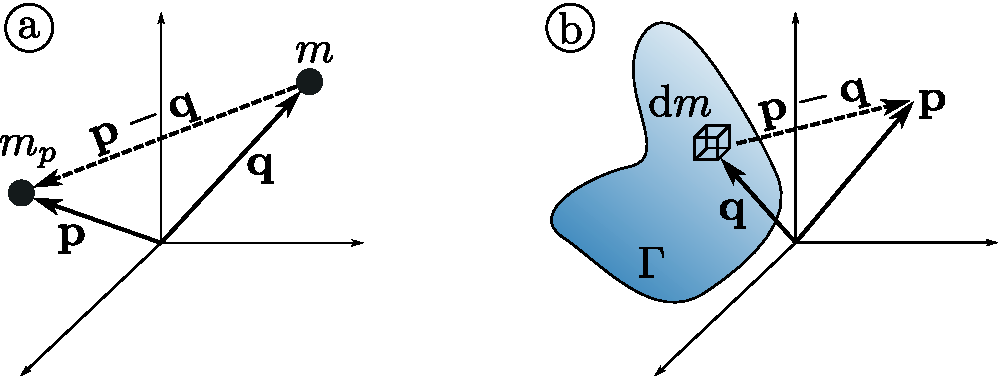
\includegraphics[width=\linewidth]{figs/gravity-potentials.pdf}
    \caption{
        (a)~Masas puntuales $m_p$ y $m$ localizadas en $\mathbf{p}$
        y $\mathbf{q}$, respectivamente.
        (b)~Distribución de masa $\Gamma$, diferencial de masa $\diff m$
        ubicado en el punto $\mathbf{q}$.
    }
    \label{fig:potencial-gravitatorio}
\end{figure}


\subsection{Potencial gravitatorio producido por una distribución de masa}

Partiendo de que un diferencial de masa $\diff m$ ubicado en $\mathbf{q}$
genera un potencial gravitatorio $\diff V$ en cualquier punto $\mathbf{p}$
(Fig.~\ref{fig:potencial-gravitatorio}b):

\begin{equation}
    \diff V(\mathbf{p}) = \frac{G}{|\mathbf{p} - \mathbf{q}|} \diff m,
\end{equation}

\noindent el potencial gravitatorio generado por una distribución de masa
$\Gamma$ puede calcularse integrando los diferenciales de masa que lo componen:

\begin{equation}
    V(\mathbf{p}) =
        G \int\limits_\Gamma \frac{\diff m}{|\mathbf{p} - \mathbf{q}|} .
\end{equation}

Si reescribimos los diferenciales de masa como

\begin{equation}
    \diff m = \rho(\mathbf{q}) \diff v,
\end{equation}

\noindent donde $\rho(\mathbf{q})$ es la densidad de masa de la distribución
$\Gamma$ en el punto $\mathbf{q}$ y $\diff v$ es el diferencial de volumen,
el potencial se puede expresar como:

\begin{equation}
    V(\mathbf{p}) =
        G \int\limits_\Gamma
        \frac{\rho(\mathbf{q})}{|\mathbf{p} - \mathbf{q}|} \diff v.
    \label{eq:potencial-gravitatorio-integral}
\end{equation}


\subsection{Gradiente del potencial gravitatorio}

Según la definición del potencial gravitatorio expuesta en la
ecuación~\ref{eq:potencial-gravitatorio-definicion}, es posible calcular la
aceleración de la gravedad producida por una distribución de masa arbitraria
en cualquier punto $\mathbf{p}$ como el gradiente del potencial
$V(\mathbf{p})$.
Si definimos un sistema de ejes Cartesianos en el cual el punto $\mathbf{p}
= (x, y, z)$, las componentes de la aceleración en cada una de las direcciones
del sistema quedan expresadas
como:

\begin{equation}
    g_i(\mathbf{p}) = \frac{\partial V(\mathbf{p})}{\partial i}, \,\,
        \forall i \in \{x, y, z\}.
    \label{eq:componentes-aceleracion-gravitatoria}
\end{equation}

El vector
$\mathbf{g}(\mathbf{p}) = (g_x(\mathbf{p}), g_y(\mathbf{p}), g_z(\mathbf{p}))$
representa la aceleración gravitatoria en el punto
$\mathbf{p}$ generada por la distribución de masa $\Gamma$, aunque es común
referirse al mismo como el \emph{gradiente gravitatorio}.
Reemplazando la ecuación~\ref{eq:potencial-gravitatorio-integral}
en~\ref{eq:componentes-aceleracion-gravitatoria}, las componentes del gradiente
gravitatorio pueden expresarse como:

\begin{align}
    g_x(\mathbf{p}) &=
        - G \int\limits_\Gamma \rho(\mathbf{q})
        \frac{(x - x')}{|\mathbf{p} - \mathbf{q}|^3} \diff v,
    \label{eq:gx-integral}
    \\
    g_y(\mathbf{p}) &=
        - G \int\limits_\Gamma \rho(\mathbf{q})
        \frac{(y - y')}{|\mathbf{p} - \mathbf{q}|^3} \diff v,
    \label{eq:gy-integral}
    \\
    g_z(\mathbf{p}) &=
        - G \int\limits_\Gamma \rho(\mathbf{q})
        \frac{(z - z')}{|\mathbf{p} - \mathbf{q}|^3} \diff v,
    \label{eq:gz-integral}
\end{align}

\noindent donde $\mathbf{q} = (x', y', z')$.

Las segundas derivadas del potencial gravitatorio definen el \emph{tensor del
gradiente gravitatorio}, y sus componentes pueden expresarse como:

\begin{equation}
    g_{ij}(\mathbf{p}) =
        \frac{\partial^2 V(\mathbf{p})}{\partial i \partial j}, \,\,
        \forall i \in \{x, y, z\}, \,\,
        \forall j \in \{x, y, z\}.
\end{equation}

Reemplazando la ecuación \ref{eq:potencial-gravitatorio-integral}, podemos
expresar las componentes diagonales del tensor de la siguiente manera
\citep{grombein2013}:

\begin{align}
    g_{xx}(\mathbf{p}) &=
        G \int\limits_\Gamma \rho(\mathbf{q})
        \left[
        \frac{3(x - x')^2}{|\mathbf{p} - \mathbf{q}|^5}
        - \frac{1}{|\mathbf{p} - \mathbf{q}|^3}
        \right]
        \diff v,
    \label{eq:gxx-integral}
    \\
    g_{yy}(\mathbf{p}) &=
        G \int\limits_\Gamma \rho(\mathbf{q})
        \left[
        \frac{3(y - y')^2}{|\mathbf{p} - \mathbf{q}|^5}
        - \frac{1}{|\mathbf{p} - \mathbf{q}|^3}
        \right]
        \diff v,
    \label{eq:gyy-integral}
    \\
    g_{zz}(\mathbf{p}) &=
        G \int\limits_\Gamma \rho(\mathbf{q})
        \left[
        \frac{3(z - z')^2}{|\mathbf{p} - \mathbf{q}|^5}
        - \frac{1}{|\mathbf{p} - \mathbf{q}|^3}
        \right]
        \diff v,
    \label{eq:gzz-integral}
\end{align}

\noindent mientras que las componentes no diagonales pueden expresarse como:

\begin{align}
    g_{xy}(\mathbf{p}) =
    g_{yx}(\mathbf{p}) &=
        G \int\limits_\Gamma \rho(\mathbf{q})
        \frac{3(x - x')(y - y')}{|\mathbf{p} - \mathbf{q}|^5}
        \diff v,
    \label{eq:gxy-integral}
    \\
    g_{xz}(\mathbf{p}) =
    g_{zx}(\mathbf{p}) &=
        G \int\limits_\Gamma \rho(\mathbf{q})
        \frac{3(x - x')(z - z')}{|\mathbf{p} - \mathbf{q}|^5}
        \diff v,
    \label{eq:gxz-integral}
    \\
    g_{yz}(\mathbf{p}) =
    g_{zy}(\mathbf{p}) &=
        G \int\limits_\Gamma \rho(\mathbf{q})
        \frac{3(y - y')(z - z')}{|\mathbf{p} - \mathbf{q}|^5}
        \diff v.
    \label{eq:gyz-integral}
\end{align}

A partir de las ecuaciones~\ref{eq:gxx-integral}--\ref{eq:gzz-integral} podemos
calcular el Laplaciano del potencial gravitatorio:

\begin{equation}
    \nabla^2 V(\mathbf{p}) =
        \frac{\partial^2 V}{\partial x^2}
        + \frac{\partial^2 V}{\partial y^2}
        + \frac{\partial^2 V}{\partial z^2},
\end{equation}

\noindent Dado que las tres expresiones se cancelan mutuamente
\citep{blakely1995}, podemos concluir que cualquier potencial gravitatorio es
un \emph{campo harmónico}

\begin{equation}
    \nabla^2 V(\mathbf{p}) = 0
    \label{eq:potencial-laplace}
\end{equation}

\noindent para cualquier punto de observación $\mathbf{p}$ fuera de la
distribución de masa $\Gamma$.

Vale notar que la ecuación de Laplace \ref{eq:potencial-laplace} es válida
solo para regiones libres de masas, y representa un caso particular de la
ecuación de Poisson \citep{blakely1995}:

\begin{equation}
    \nabla^2 V(\mathbf{p}) = -4\pi G \rho,
    \label{eq:potencial-poisson}
\end{equation}

\noindent válida para cualquier punto de observación $\mathbf{p}$.

% =============================================================================

\section{Modelado directo}

El cálculo de los efectos gravitatorios de un determinado cuerpo sobre uno
o más puntos de observación se suele denominar modelado directo (\emph{forward
modelling} en inglés).
Aunque las expresiones del potencial gravitatorio
(ec.~\ref{eq:potencial-gravitatorio-integral}),
las componentes de su gradiente
(ecs.~\ref{eq:gx-integral}--\ref{eq:gz-integral})
y de su tensor (ecs.~\ref{eq:gxx-integral}--\ref{eq:gzz-integral}
aparentan ser sencillas, el cómputo de estas magnitudes para una geometría dada
no resulta un problema trivial.
Solo existen soluciones analíticas a dichas expresiones para determinadas
geometrías sencillas o que guardan algún tipo de simetría.

En el desarrollo de esta Tesis nos resultan de principal interés trabajar con
tres tipos de geometrías: masas puntuales, prismas rectangulares y prismas
esféricos o \emph{tesseroides}.

\subsection{Masas puntuales}

La distribución de densidades de una masa puntual puede expresarse
sencillamente mediante una Delta de Dirac \citep{vladimirov1979}:

\begin{equation}
    \rho(\mathbf{q}) = m \, \delta(\mathbf{q} - \mathbf{q'}),
\end{equation}

\noindent donde $\mathbf{q}$ y $m$ son la posición y la masa de la partícula,
respectivamente.
Reemplazando esta expresión en la
ecuación~\ref{eq:potencial-gravitatorio-integral}, obtenemos el potencial
gravitatorio generado por una partícula:

\begin{equation}
    V(\mathbf{p}) =
        G \int\limits_\Gamma
        m \frac{\delta(\mathbf{q} - \mathbf{q'})}{|\mathbf{p} - \mathbf{q'}|}
        \diff v =
        \frac{G m}{|\mathbf{p} - \mathbf{q}|},
    \label{eq:potencial-masa-puntual}
\end{equation}

\noindent de acuerdo con la expresión del potencial de la
ecuación~\ref{eq:potencial-gravitatorio-particula}.

Realizando el mismo reemplazos en las ecuaciones correspondientes a las
componentes del gradiente (ecs.~\ref{eq:gx-integral}--\ref{eq:gz-integral})
arribamos a las siguientes expresiones:

\begin{align}
    g_x(\mathbf{p}) &=
        - G m
        \frac{x - x'}{|\mathbf{p} - \mathbf{q}|^3},
    \label{eq:gx-particula}
    \\
    g_y(\mathbf{p}) &=
        - G m
        \frac{y - y'}{|\mathbf{p} - \mathbf{q}|^3},
    \label{eq:gy-particula}
    \\
    g_z(\mathbf{p}) &=
        - G m
        \frac{z - z'}{|\mathbf{p} - \mathbf{q}|^3}.
    \label{eq:gz-particula}
\end{align}

A la hora de realizar el cómputo de los campos gravitatorios de masas
puntuales, las posiciones de las partículas como de los puntos de observación
pueden venir dados en diferentes sistemas de coordenadas.
En el caso de necesitar modelar cualquier conjunto de masas situadas bajo la
superficie terrestre, resulta natural utilizar coordenadas esféricas tanto para
las posiciones de las partículas como para los puntos de observación.
Sin embargo, es muy común trabajar sobre zonas de estudio con dimensiones
acotadas, bajo las cuales la aproximación de tierra plana es suficiente. En
estos casos es posible trabajar en coordenadas Cartesianas.

\subsubsection{Coordenadas Cartesianas}

En el caso de que la posición de la partícula venga dada por el vector
$\mathbf{q} = (x', y', z')$ y el punto de observación por el vector
$\mathbf{p} = (x, y, z)$ definidos en el mismo sistema de ejes Cartesianos, el
módulo de
$\mathbf{p} - \mathbf{q}$ se calcula sencillamente bajo la norma L$_2$:

\begin{equation}
    | \mathbf{p} - \mathbf{q} | = \sqrt{
        (x - x')^2 + (y - y')^2 + (z - z')^2
    }.
\end{equation}

Dado que los numeradores en las
ecuaciones~\ref{eq:gx-particula}--\ref{eq:gz-particula} resultan triviales en
coordenadas Cartesianas, el cómputo del potencial y las componentes de su
gradiente se puede realizar de manera sencilla.

\subsubsection{Coordenadas esféricas}

Consideremos que las posiciones del punto de observación y de la partícula
vienen dados en un sistema de coordenadas esféricas. Para ello vamos a definir
un sistema de referencia \emph{geocéntrico} $\{X, Y, Z\}$ y a partir del mismo
un sistema de coordenadas esféricas $\{r, \lambda, \phi\}$, donde $r$ es la
posición \emph{radial}, $\lambda$ la posición \emph{longitudinal} y $\phi$ la
posición \emph{latitudinal} (Fig.~\ref{fig:spherical-coordinates}).
Cualquier punto dado por las coordenadas esféricas $(r, \lambda, \phi)$ se
puede expresar en coordenadas Cartesianas geocéntricas bajo las siguientes
relaciones:

\begin{equation}
    \begin{cases}
        X = r \cos\lambda \cos{\phi} \\
        Y = r \sin\lambda \cos{\phi} \\
        Z = r \sin{\phi},
    \end{cases}
\end{equation}

\noindent donde $r \in [0, \infty)$, $\lambda \in (-\pi, \pi]$ y
$\phi \in [-\pi/2, \pi/2]$.

\begin{figure}
    \centering
    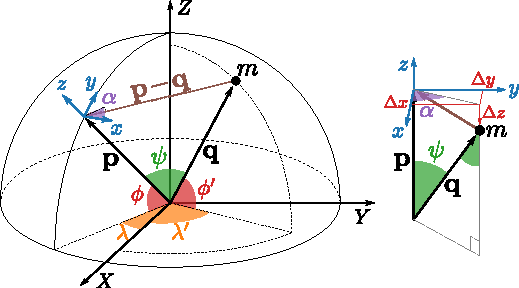
\includegraphics[width=\linewidth]{figs/spherical-coordinates.pdf}
    \caption{
        Masa puntual $m$ ubicada en la posición $\mathbf{q}$ y punto de
        observación situado en $\mathbf{p}$.
        Se define un sistema de referencia Cartesiano \emph{geocéntrico} $X, Y,
        Z$ bajo el cual se considera un sistema de coordenadas esféricas dadas
        por la distancia radial ($r$), ángulo longitudinal ($\lambda$) y ángulo
        latitudinal ($\phi$).
        En el punto $\mathbf{p}$ se define un sistema \emph{local} de
        coordenadas Cartesiano: el eje $x$ apunta hacia el Este,
        el eje $y$ hacia el Norte geométrico y el eje $z$ en la dirección
        radial.
        Se define a $\psi$ como el ángulo descripto por los vectores
        $\mathbf{p}$ y $\mathbf{q}$, y $\alpha$ al ángulo azimutal de
        $-(\mathbf{p} - \mathbf{q})$ sobre el sistema \emph{local}.
    }
    \label{fig:spherical-coordinates}
\end{figure}

El potencial gravitatorio que genera la partícula $m$ sobre el punto de
observación $\mathbf{p}$ puede calcularse mediante la
ecuación~\ref{eq:potencial-gravitatorio-particula}.
Considerando que los vectores $\mathbf{p}$ y $\mathbf{q}$ vienen definidos por
las coordenadas esféricas $(r, \lambda, \phi)$ y $(r', \lambda', \phi')$,
respectivamente, la distancia Euclidiana entre ellos puede expresarse como
\citep{grombein2013}:

\begin{equation}
    |\mathbf{p} - \mathbf{q}| = \sqrt{
        r^2 + r'^2 - 2rr'\cos\psi
    },
    \label{eq:distance-spherical}
\end{equation}

\noindent donde $\psi$ es el ángulo que describen los vectores $\mathbf{p}$
y $\mathbf{q}$:

\begin{equation}
    \cos \psi =
        \sin \phi \sin \phi' + \cos \phi \cos \phi' \cos(\lambda - \lambda').
    \label{eq:cosphi}
\end{equation}

La determinación de las componentes del gradiente del potencial gravitatorio
hace necesario que definamos las direcciones ortogonales $x$, $y$ y $z$ a lo
largo de las cuales se calculan las derivadas parciales de $V(\mathbf{p})$.
La elección más natural es obtener el gradiente con respecto a un sistema de
coordenadas \emph{local} $\{x, y, z\}$ \citep{grombein2013,uieda2016} donde $x$
se orienta en la dirección longitudinal (Este), $y$ en la dirección latitudinal
(Norte) y $z$ en la dirección radial.

Los numeradores de las ecuaciones~\ref{eq:gx-particula}--\ref{eq:gz-particula}
pueden expresarse en términos de las coordenadas esféricas como:

\begin{align}
    \Delta x &= - (x - x') = r' \sin\psi \cos\alpha
    \label{eq:delta-x-raw}
    \\
    \Delta y &= - (y - y') = r' \sin\psi \sin\alpha
    \label{eq:delta-y-raw}
    \\
    \Delta z &= - (z - z') = r'\cos\psi - r,
    \label{eq:delta-z-raw}
\end{align}

\noindent donde $\alpha$ es el ángulo azimutal del vector
$-(\mathbf{p} - \mathbf{q})$ sobre el sistema de coordenadas \emph{locales}.
Haciendo uso de las siguientes relaciones de trigonometría esférica
\citep[][p.~113]{heiskanen1967}:

\begin{align}
    \sin\psi \cos\alpha &=
        \cos\phi \sin\phi' - \sin\phi \cos\phi' \cos(\lambda - \lambda') \\
    \sin\psi \sin\alpha &=
        \cos\phi' \sin(\lambda - \lambda'),
\end{align}

\noindent podemos expresar las ecuaciones~\ref{eq:delta-x-raw},
\ref{eq:delta-y-raw} y \ref{eq:delta-z-raw} como \citep{grombein2013}:

\begin{align}
    \Delta x &= r' \sin\psi \left[
        \cos\phi \sin\phi' - \sin\phi \cos\phi' \cos(\lambda - \lambda')
        \right]
    \label{eq:delta-x}
    \\
    \Delta y &= r' \cos\phi' \sin(\lambda - \lambda')
    \label{eq:delta-y}
    \\
    \Delta z &= r'\cos\psi - r.
    \label{eq:delta-z}
\end{align}

Las componentes del gradiente del potencial gravitatorio generado por una masa
puntual en coordenadas esféricas quedan determinadas de la siguiente manera:

\begin{align}
    g_x(\mathbf{p}) &=
        G m
        \frac{\Delta x}{|\mathbf{p} - \mathbf{q}|^3},
    \label{eq:gx-particula-spherical}
    \\
    g_y(\mathbf{p}) &=
        G m
        \frac{\Delta y}{|\mathbf{p} - \mathbf{q}|^3},
    \label{eq:gy-particula-spherical}
    \\
    g_z(\mathbf{p}) &=
        G m
        \frac{\Delta z}{|\mathbf{p} - \mathbf{q}|^3},
    \label{eq:gz-particula-spherical}
\end{align}

\noindent haciendo uso de las ecuaciones~\ref{eq:distance-spherical},
\ref{eq:cosphi}, \ref{eq:delta-x}, \ref{eq:delta-y} y \ref{eq:delta-z}.


\subsection{Prismas rectangulares}

A la hora de modelar estructuras tridimensionales subyacentes a la superficie
terrestre, los primas rectangulares se presentan como la geometría a elección
por parte de muchos autores y muchas autoras \citep{}.
Una de las razones recae en la simpleza de la geometría, aunque una que no
debemos obviar es el hecho de que existen soluciones analíticas a las
ecuaciones de los campos gravitatorios generados por prismas rectangulares
\citep{nagy2000,nagy2002}.

Consideremos un prisma rectangular de densidad homogénea $\rho$ cuyos vértices
se encuentran determinados por las coordenadas $X_1, X_2, Y_1, Y_2, Z_1, Z_2$
definidas en un sistema de ejes Cartesianos ${X, Y, Z}$
(Fig.~\ref{fig:rectangular-prism}).
El potencial gravitatorio que genera el prisma sobre un punto de observación
$\mathbf{p} = (X, Y, Z)$ definido en el sistema ${X, Y, Z}$ se puede
calcular mediante la ecuación~\ref{eq:potencial-gravitatorio-integral},
reemplazando el dominio de integración:

\begin{equation}
    V(\mathbf{p}) =
    G \rho
    \int\limits_{X_1}^{X_2}
    \int\limits_{Y_1}^{Y_2}
    \int\limits_{Z_1}^{Z_2}
    \frac{\diff X' \diff Y' \diff Z'}{|\mathbf{p} - \mathbf{q}|},
\end{equation}

\noindent donde

\begin{equation}
    |\mathbf{p} - \mathbf{q}| = \sqrt{
        (X - X')^2 + (Y - Y')^2 + (Z - Z')^2
    }.
\end{equation}

\begin{figure}
    \centering
    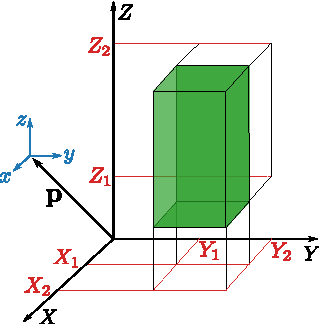
\includegraphics[width=0.6\linewidth]{figs/rectangular-prism.pdf}
    \caption{
        Prisma rectangular y punto de observación $\mathbf{p}$ definidos en un
        sistema de coordenadas Cartesianas $\{X, Y, Z\}$. Se define un sistema
        de coordenadas Cartesianas $\{x, y, z\}$ con origen en el punto de
        observación $\mathbf{p}$ y con ejes paralelos a $X, Y, Z$,
        respectivamente.
    }
    \label{fig:rectangular-prism}
\end{figure}

Con el objetivo de simplificar los cálculos, definimos un sistema de
coordenadas Cartesianas $\{x, y, z\}$ cuyo origen se encuentra en el punto de
observación $\mathbf{p}$ y sus ejes son paralelos a los del sistema $\{X, Y,
Z\}$, respectivamente (Fig.~\ref{fig:rectangular-prism}).
Los vértices del prisma vendrán dados por las coordenadas
$x_1, x_2, y_1, y_2, z_1, z_2$ en el nuevo sistema de referencia, es decir:

\begin{equation}
    \begin{aligned}
        x_1 &= X_1 - X, & x_2 &= X_2 - X, \\
        y_1 &= Y_1 - Y, & y_2 &= Y_2 - Y, \\
        z_1 &= Z_1 - Z, & z_2 &= Z_2 - Z.
    \end{aligned}
\end{equation}

Bajo este nuevo sistema de referencia, el potencial gravitatorio se puede
expresar como:

\begin{equation}
    V(\mathbf{p}) =
    G \rho
    \int\limits_{x_1}^{x_2}
    \int\limits_{y_1}^{y_2}
    \int\limits_{z_1}^{z_2}
    \frac{\diff x' \diff y' \diff z'}{\sqrt{{x'}^2 + {y'}^2 + {z'}^2}}.
\end{equation}

El resultado de esta integración posee la siguiente forma
\citep{nagy2000,nagy2002}:

\begin{equation}
    \begin{split}
        V(\mathbf{p}) =
        G \rho
        \Bigg[ &
            xy \ln (z + l) + yz \ln(x + l) + zx \ln(y + l) \\
               &
            - \frac{x^2}{2} \arctan \frac{yz}{xl}
            - \frac{y^2}{2} \arctan \frac{zx}{yl}
            - \frac{z^2}{2} \arctan \frac{xy}{zl}
        \Bigg]
        \Bigg|_{x_1}^{x_2}
        \Bigg|_{y_1}^{y_2}
        \Bigg|_{z_1}^{z_2},
    \end{split}
    \label{eq:potencial-prismas-analitico}
\end{equation}

\noindent donde

\begin{equation}
    l = \sqrt{x^2 + y^2 + z^2}.
\end{equation}

Reemplazando todos los límites del dominio de integración, obtenemos un total
de 48 términos.
A la hora de evaluarlos numéricamente hay que tener en cuenta que la solución
analítica de la ecuación~\ref{eq:potencial-prismas-analitico} no es
continua en todo $\mathbb{R}^3$, particularmente en los casos en los que el
punto de observación se encuentra sobre alguno de los vértices, aristas o caras
del prisma ($x_{1,2}=0$, $y_{1,2}=0$ ó $z_{1,2}=0$). Sin embargo el potencial
$V(\mathbf{p})$ sí lo es.
Para solucionar esto, es necesario reemplazar aquellos términos que no pueden
ser evaluados por sus límites cuando $(x, y, z) \rightarrow (0, 0, 0)$
\citep{nagy2000}.
Por ejemplo:

\begin{equation}
    \lim_{(x, y, z)\rightarrow (0, 0, 0)} xz \ln(z + r) = 0.
\end{equation}

Una solución es definir una nueva función $\safelog(x)$ de la siguiente
manera:

\begin{equation}
    \safelog(x) =
    \begin{cases}
        \ln(x) & \quad x \ge x_\text{umbral} \\
        0      & \quad x < x_\text{umbral}
    \end{cases}
    \label{eq:safe_log}
\end{equation}

\noindent donde $x_\text{umbral}$ es un valor muy pequeño del argumento de
$\safelog$ a partir del cual consideramos que la función debe ser evaluada en
su límite en cero.
La elección de este valor dependerá de las dimensiones del problema que estamos
resolviendo.
En el caso de un modelado directo geofísico, en el cual las dimensiones de los
primas vienen dadas por varios metros, podemos asumir un valor de
$x_\text{umbral} = 10^{-10}$m \citep{harmonica2021}.

Por otro lado, la evaluación de la función $\arctan$ requiere ciertos cuidados.
Para que el potencial $V(\mathbf{p})$ satisfaga la ecuación de Poisson
(ec.~\ref{eq:potencial-poisson}), es necesario utilizar la siguiente forma de
la función $\safearctan(y, x)$ \citep{fukushima2020}:

\begin{equation}
    \safearctan(y, x) =
    \begin{cases}
        \arctan(y / x) & \quad x \ne 0 \\
        \pi / 2        & \quad x = 0,\, y > 0 \\
        -\pi / 2       & \quad x = 0,\, y < 0 \\
        0              & \quad x = 0,\, y = 0.
    \end{cases}
    \label{eq:safe_arctan}
\end{equation}

Haciendo uso de las funciones $\safelog$ y $\safearctan$ definidas en las
ecuaciones~\ref{eq:safe_log} y \ref{eq:safe_arctan}, respectivamente, el
potencial gravitatorio generado por un prisma rectangular en cualquier punto de
observación $\mathbf{p}$ puede ser numéricamente calculado mediante:

\begin{equation}
    \begin{split}
        V(\mathbf{p}) =
        G \rho
        \Bigg[ &
            xy \safelog (z + l)
            + yz \safelog(x + l)
            + zx \safelog(y + l)
           - \frac{x^2}{2} \safearctan(yz, xl)
                \\&
           - \frac{y^2}{2} \safearctan(zx, yl)
           - \frac{z^2}{2} \safearctan(xy, zl)
        \Bigg]
        \Bigg|_{x_1}^{x_2}
        \Bigg|_{y_1}^{y_2}
        \Bigg|_{z_1}^{z_2}.
    \end{split}
    \label{eq:potencial-prismas-numerico}
\end{equation}

De manera análoga, podemos calcular las componentes del gradiente del potencial
gravitatorio generado por un prisma rectangular haciendo uso de las siguientes
expresiones \citep{nagy2000,nagy2002}:

\begin{align}
    g_x(\mathbf{p}) =&
        \Big[
            y \safelog(z + l) + z \safelog(y + l)  - x \safearctan(yz, xl)
        \Big]
        \Big|_{x_1}^{x_2}
        \Big|_{y_1}^{y_2}
        \Big|_{z_1}^{z_2} \\
    g_y(\mathbf{p}) =&
        \Big[
            z \safelog(x + l) + x \safelog(z + l)  - y \safearctan(zx, yl)
        \Big]
        \Big|_{x_1}^{x_2}
        \Big|_{y_1}^{y_2}
        \Big|_{z_1}^{z_2} \\
    g_z(\mathbf{p}) =&
        \Big[
            x \safelog(y + l) + y \safelog(x + l) - z \safearctan(xy, zl)
        \Big]
        \Big|_{x_1}^{x_2}
        \Big|_{y_1}^{y_2}
        \Big|_{z_1}^{z_2}.
\end{align}


\subsection{Tesseroides}

En caso de querer realizar modelos directos de estructuras regionales,
continentales o globales,
El uso de prismas rectangulares en coordenadas Cartesianas no resulta la mejor
opción, ya que no tienen en cuenta la curvatura del planeta Tierra.
La mayoría de los modelos directos que sí lo hacen se definen en coordenadas
esféricas geocéntricas y consisten en discretizar la Tierra en geometrías
simples.
Este es el caso de los tesseroides \citep{anderson1976}, también conocidos como
prismas esféricos, los cuales se definen como el volumen comprendido entre dos
esferas de radios distintos, dos meridianos de longitudes distintas y dos
paralelos de distintas latitudes (Fig.~\ref{fig:tesseroid}).

\begin{figure}
    \centering
    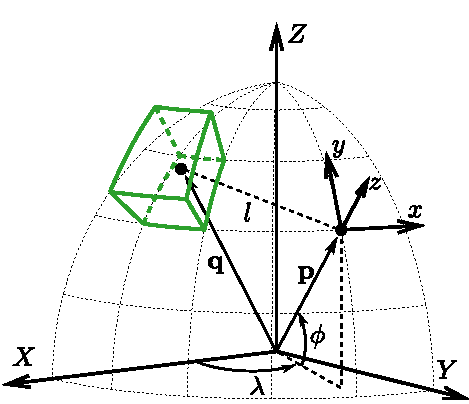
\includegraphics[width=0.7\linewidth]{figs/tesseroid-coord-sys.pdf}
    \caption{
        Tesseroide (prisma esférico) en un sistema de coordenadas esféricas
        geocéntricas, junto a un punto de cómputo situado en $\mathbf{p}$ y su
        correspondiente sistema \emph{local} de coordenadas Cartesianas.
        Obtenida de \citet{uieda2015}.
    }
    \label{fig:tesseroid}
\end{figure}

El potencial gravitatorio que genera un tesseroide de densidad uniforme $\rho$,
definido por las coordenadas $r_1$, $r_2$, $\lambda_1$, $\lambda_2$, $\phi_1$
y $\phi_2$, sobre un punto de observación $\mathbf{p}$ dado por las coordenadas
esféricas $r$, $\lambda$ y $\phi$ se puede obtener aplicando estos límites de
integración a la ecuación~\ref{eq:potencial-gravitatorio-integral}, quedando
expresado como la siguiente integral volumétrica
\citep{grombein2013,uieda2016}:

\begin{equation}
    V(\mathbf{p}) = G \rho
        \int\limits_{r_1}^{r_2}
        \int\limits_{\lambda_1}^{\lambda_2}
        \int\limits_{\phi_1}^{\phi_2}
        \frac{\kappa}{|\mathbf{p} - \mathbf{q}|}
        \diff r' \diff \lambda' \diff \phi',
    \label{eq:potencial-tesseroide}
\end{equation}

\noindent donde

\begin{equation}
    \kappa = {r'}^2 \cos \phi',
    \label{eq:kappa}
\end{equation}

\noindent la distancia $|\mathbf{p} - \mathbf{q}|$ viene dada por la
ecuación~\ref{eq:distance-spherical} y las coordenadas de integración $r'$,
$\lambda'$ y $\phi'$ representan la posición $\mathbf{q}$ de cada volumen
infinitesimal del tesseroide.

Reemplazando los límites de integración del tesseroide en las ecuaciones
\ref{eq:gx-integral}, \ref{eq:gy-integral} y \ref{eq:gz-integral} podemos
obtener las componentes del gradiente del potencial gravitatorio generado por
el tesseroide en el punto de observación $\mathbf{p}$ tomando las derivadas
parciales con respecto al sistema de coordenadas \emph{local}:


\begin{align}
    g_x(\mathbf{p}) &=
        G \rho
        \int\limits_{r_1}^{r_2}
        \int\limits_{\lambda_1}^{\lambda_2}
        \int\limits_{\phi_1}^{\phi_2}
        \frac{\Delta x}{|\mathbf{p} - \mathbf{q}|^3}
        \kappa
        \diff r' \diff \lambda' \diff \phi',
    \label{eq:gx-tesseroide}
    \\
    g_y(\mathbf{p}) &=
        G \rho
        \int\limits_{r_1}^{r_2}
        \int\limits_{\lambda_1}^{\lambda_2}
        \int\limits_{\phi_1}^{\phi_2}
        \frac{\Delta y}{|\mathbf{p} - \mathbf{q}|^3}
        \kappa
        \diff r' \diff \lambda' \diff \phi',
    \label{eq:gy-tesseroide}
    \\
    g_z(\mathbf{p}) &=
        G \rho
        \int\limits_{r_1}^{r_2}
        \int\limits_{\lambda_1}^{\lambda_2}
        \int\limits_{\phi_1}^{\phi_2}
        \frac{\Delta z}{|\mathbf{p} - \mathbf{q}|^3}
        \kappa
        \diff r' \diff \lambda' \diff \phi',
    \label{eq:gz-tesseroide}
\end{align}

\noindent donde $\Delta x$, $\Delta y$ y $\Delta z$ vienen dadas por las
ecuaciones~\ref{eq:delta-x}, \ref{eq:delta-y} y \ref{eq:delta-z},
respectivamente.

Las ecuaciones~\ref{eq:potencial-tesseroide}, \ref{eq:gx-tesseroide},
\ref{eq:gy-tesseroide} y \ref{eq:gz-tesseroide} contienen integrales elípticas
que no poseen solución analítica y deben ser aproximadas numéricamente.
Existen dos principales métodos en la literatura para aproximar estas
integrales: uno involucra expansiones en serie de Taylor
\citep{heck2006,grombein2013} mientras que los otros hacen uso de la \ac{GLQ}
\citep{asgharzadeh2007,wildpfeiffer2008,li2011,uieda2016,lin2018}.
En el Capítulo~\ref{cha:tesseroids-variable-density} se detalla las razones por
las cuales a lo largo de esta Tesis abordaremos la estrategia de \ac{GLQ}.

La \Ac{GLQ} consiste en la aproximación de una integral por una suma ponderada
del kernel de integración \citep[][p.~390]{hildebrand1987}:

\begin{equation}
    \int\limits_{-1}^1 f(x) \diff x \approx
        \sum\limits_{i=1}^{N} W_i f(x_i),
\end{equation}

\noindent donde $N$ es el orden de la cuadratura,
$x_i$ corresponden a las raíces del polinomio de Legendre $P_N(x)$ de grado $N$
y $W_i$ son los pesos ponderados de cada término:

\begin{equation}
    W_i = \frac{2}{(1 - x_i^2) \Big[ P'_N(x_i) \Big]^2}.
\end{equation}

\noindent El polinomio de Legendre $P_N(x)$ y su primera derivada $P'_N(x)$ se
pueden obtener mediante relaciones de recurrencia \citep[][p.~330]{hildebrand1987}:

\begin{align}
    &P_0(x) = 1 \\
    &P_1(x) = x \\
    &P_{m + 1}(x) = \frac{2m + 1}{m + 1} x P_m(x) - \frac{m}{m + 1}P_{m-1}(x).
\end{align}

La Tabla~\ref{tab:legendre-roots} muestra las raíces de los primeros polinomios
de Legendre y sus respectivos pesos ponderados.

\begin{table}
    \centering
    \caption{
        Raíces de algunos polinomios de Legendre junto con los correspondientes
        pesos ponderados a ser utilizados en la \ac{GLQ}
        \citep[][p.~392]{hildebrand1987}.
    }
    \begin{tabular}{ccc}
        \hline
        Orden ($N$) & Raíces ($x_i$)                                     & Pesos ponderados ($W_i$)    \\
        \hline
        1     & 0                                                        & 2                           \\
        2     & $\pm \frac{1}{\sqrt{3}}$                                 & 1                           \\
        3     & 0                                                        & $\frac{8}{9}$               \\
              & $\pm \sqrt{\frac{3}{5}}$                                 & $\frac{5}{9}$               \\
        4     & $\pm \sqrt{\frac{3}{7} - \frac{2}{7}\sqrt{\frac{6}{5}}}$ & $\frac{18 + \sqrt{30}}{36}$ \\
              & $\pm \sqrt{\frac{3}{7} + \frac{2}{7}\sqrt{\frac{6}{5}}}$ & $\frac{18 - \sqrt{30}}{36}$
    \end{tabular}
    \label{tab:legendre-roots}
\end{table}

En el caso de que la integral posea límites de integración distintos a
$[-1, 1]$, podemos escalar los nodos y aplicar la \ac{GLQ} de la siguiente
forma:

\begin{equation}
    \int\limits_a^b f(x) \diff x \approx
        \frac{b - a}{2} \sum\limits_{i=1}^{N}
        W_i f(x_i^s),
\end{equation}

\noindent donde

\begin{equation}
    x_i^s = \frac{b - a}{2} x_i + \frac{b + a}{2}.
\end{equation}

Haciendo uso de la \ac{GLQ}, podemos aproximar las integrales volumétricas de
las ecuaciones~\ref{eq:potencial-tesseroide}, \ref{eq:gx-tesseroide},
\ref{eq:gy-tesseroide}, \ref{eq:gz-tesseroide} de la siguiente manera
\citep{asgharzadeh2007,uieda2016}:

\begin{equation}
    \int\limits_{r_1}^{r_2}
    \int\limits_{\lambda_1}^{\lambda_2}
    \int\limits_{\phi_1}^{\phi_2}
    f(r', \lambda', \phi')
    \diff r' \diff \lambda' \diff \phi' =
    A
    \sum\limits_{i=1}^{N_r}
    \sum\limits_{j=1}^{N_\lambda}
    \sum\limits_{k=1}^{N_\phi}
    W_i^r
    W_j^\lambda
    W_k^\phi
    f(r_i, \lambda_j, \phi_j),
    \label{eq:glq-integral-volumetrica}
\end{equation}

\noindent donde

\begin{equation}
    A = \frac{
        (r_2 - r_1) (\lambda_2 - \lambda_1) (\phi_2 - \phi_1)
    }{8},
\end{equation}

\noindent $N_r$, $N_\lambda$ y $N_\phi$ son los ordenes de la cuadratura en
cada dirección; $r_i$, $\lambda_j$ y $\phi_k$ representan los nodos escalados
de las cuadraturas para cada dirección; y $W_i^r$, $W_j^\lambda$, $W_k^\phi$
sus respectivos pesos ponderados.

Como se puede observar en la ecuación~\ref{eq:glq-integral-volumetrica}, la
\ac{GLQ} aproxima los campos gravitatorios de un tesseroide por los que genera
un conjunto de masas puntuales situadas en los nodos escalados de los
polinomios de Legendre.
La precisión de la aproximación dependerá entonces de la cantidad de nodos
utilizados en las sumatorias, es decir, de los ordenes de las cuadraturas.
De esta forma podemos aumentar la precisión de la \ac{GLQ} incrementando los
ordenes de las cuadraturas.
Sin embargo, el aumento de cada cuadratura incrementa la cantidad de nodos
según $O(n^3)$, haciendo de esta estrategia un método muy ineficiente.

\citet{ku1977} demostró que la precisión de la aproximación también depende del
cociente entre la distancia al punto de observación y la distancia entre nodos
adyacentes.
Haciendo uso de esto, \citet{li2011} han propuesto un método más eficiente para
aumentar la precisión de la aproximación manteniendo: la \emph{discretización
adaptativa}.
Esta consiste en mantener el orden de las cuadraturas constantes e ir
dividiendo el tesseroide en otros tesseroides de menor tamaño según la
distancia entre ellos y el punto de observación.
De esta forma, se incrementa la cantidad de nodos en las regiones que mayor
afectan a la precisión, obteniendo un número considerablemente menor de nodos
pero manteniendo una buena precisión.
En el Capítulo \ref{cha:tesseroids-variable-density} describiremos en detalle
la \emph{discretización adaptativa}.

% =============================================================================

\section{Disturbio de gravedad}

\subsection{Elipsoide de referencia}

\section{Fuentes equivalentes}


\chapter{Tesseroides de densidad variable}
\label{cha:tesseroids-variable-density}

Este Capítulo es una traducción al español del artículo titulado
\emph{Gravitational field calculation in spherical coordinates using variable
densities in depth} escrito por Santiago R. Soler, Agustina Pesce, Mario E.
Gimenez y Leonardo Uieda, y publicado en \emph{Geophysical Journal
International} en Junio de 2019 \citep{soler2019}.
Una preimpresión del artículo se encuentra disponible bajo licencia Creative
Commons Atribución 4.0 Internacional en
\href{https://eartharxiv.org/}{EarthArXiv}:
\url{https://doi.org/10.31223/osf.io/3548g}.

\section{Resumen}

Presentamos una nueva metodología para calcular los campos gravitatorios
generados por tesseroides (prismas esféricos) cuya densidad varía en
profundidad según una función continua arbitraria.
Esta metodología aproxima los campos gravitatorios mediante una \ac{GLQ} junto
con la aplicación de dos algoritmos de discretización que controlan
automáticamente la precisión de la aproximación dividiendo adaptativamente el
tesseroide original en otros más pequeños.
El primero es un algoritmo preexistente de discretización adaptativa
bidimensional que reduce el error debido a la distancia entre el tesseroide
y el punto de cómputo.
El segundo es un nuevo algoritmo de discretización basado en la densidad que
reduce los errores debido a la variación de la densidad con la profundidad.
La cantidad de subdivisiones que realiza cada algoritmo es indirectamente
controlada por dos parámetros: el \emph{ratio distancia-tamaño} y el
\emph{ratio delta}.
Hemos obtenido soluciones analíticas de los campos gravitatorios generados por
un cascarón esférico con densidades variables a lo largo de la dirección radial
y los hemos comparado con los resultados del modelo numérico para densidades
lineales, exponenciales y sinusoidales.
Las densidades oscilantes fueron utilizadas con la única intención de someter
al algoritmo a sus límites y no para emular un escenario real.
Estas comparaciones nos han permitido obtener valores óptimos para los
\emph{ratio} distancia-tamaño y \emph{delta} que garantizan una precisión de
0.1\% en relación con las soluciones analíticas.
Los valores óptimos del \emph{ratio} distancia-tamaño para el potencial
gravitatorio y su gradiente son 1 y 2.5, respectivamente.
La discretización basada en la densidad no es necesaria en los casos de
densidad lineal, pero se requiere de un \emph{ratio delta} de 0.1 para
densidades exponenciales y la mayoría de las sinusoidales.
Estos valores pueden ser extrapolados para cubrir los usos más comunes, siempre
y cuando los perfiles de densidad sean más simples que funciones sinusoidales.
Aunque los \emph{ratios} densidad-tamaño y \emph{delta} pueden ser configurados
por los usuarios o las usuarias para aumentar la precisión de los resultados
a expensas de un aumento en el tiempo de cómputo.
Por último, hemos aplicado esta nueva metodología para modelar la Cuenca
Neuquina, una cuenca de antepaís en Argentina, con una profundidad máxima de
5000\m{} y utilizando una densidad exponencial.


\section{Introducción}

La variación de la densidad de la litósfera con respecto a la profundidad ha
sido estudiada por casi un siglo.
A lo largo de este tiempo, varias relaciones entre la densidad y la profundidad
han sido propuestas para diferentes tipos de rocas
\citep[por ejemplo~][]{maxant1980, rao1986, rao1993, rao1994}.
Además, densidades que varían con la profundidad han sido utilizadas en el
modelado directo e inverso de datos gravitatorios, principalmente aplicados
a cuencas sedimentarias
\citep{cordell1973, rao1986, cowie1990, rao1993, rao1994, zhang2001,
welford2010}.
Estos modelos directos han sido desarrollados para cuerpos bidimensionales
o tridimensionales en coordenadas Cartesianas, lo que limita su aplicación
a escalas locales.
La llegada de la gravimetría satelital ha proveído mediciones del campo
gravitatorio terrestre con cobertura global, permitiendo el modelado
e interpretación en escalas regionales o globales.
Por esta razón, diseñar métodos de modelado directo que reproducen las
anomalías de gravedad para esas escalas resulta muy importante.

Con el objetivo de tomar en consideración la curvatura de la Tierra, muchos
modelos directos globales se definen en coordenadas esféricas geocéntricas
(ver Capítulo~\ref{cha:fundamentos}).
Un abordaje común es discretizar la Tierra en tesseroides (prismas esféricos)
\citep{anderson1976}, los cuales son definidos por el volumen que delimitan
pares de latitud, longitud y radios (Fig.~\ref{fig:tesseroid}).
Los campos gravitatorios generados por un tesseroide en cualquier punto
exterior vienen dados por integrales de volumen que deben ser aproximadas
numéricamente.
La literatura ofrece dos abordajes principales: uno involucra expansiones en
series de Taylor \citep{heck2006, grombein2013}, mientras que el otro hace uso
de la \ac{GLQ}.
La expansión en series de Taylor no resulta adecuada para desarrollar un
algoritmo que soporte densidades variables según funciones arbitrarias: los
diferentes términos de las series deberían obtenerse para cada una de las
posibles funciones de densidad.
Por el contrario, una función de densidad arbitraria puede incluirse dentro de
la \ac{GLQ} sin necesidad de modificar el método de integración.
Es por esta razón que haremos foco en los métodos basados en la \ac{GLQ} de
aquí en adelante.

El principal desafío de la integración por \ac{GLQ} es la pérdida de precisión
que ocurre cuando el punto de cómputo se acerca al tesseroide \citep{ku1977}.
\citet{uieda2016} desarrollaron un método a partir del algoritmo de
discretización adaptativa tridimensional de \citet{li2011} para obtener de
manera automática campos gravitatorios de tesseroides con densidad uniforme
con una precisión de 0.1\%.
El algoritmo divide recursivamente un tesseroide en otros más pequeños cuando
un determinado umbral es excedido, esto es cuando la distancia normalizada
al punto de cómputo es mayor que un parámetro denominado \emph{ratio
distancia-tamaño} ($D$).
\citet{uieda2016} obtuvieron además valores estándar de $D$ para el cómputo del
potencial gravitatorio, las componentes de su gradiente y del tensor del
gradiente comparando los resultados de la integración numérica con los campos
generados por un cascarón esférico.

Dos publicaciones recientes presentan abordajes alternativos para calcular los
campos gravitatorios de tesseroides homogéneos e incorporan metodologías para
el caso de tesseroides con densidades variables en profundidad.
\citet{fukushima2018} ha resuelto analíticamente la integral correspondiente al
potencial gravitatorio en la dirección radial, obteniendo una integral de
superficie, la cual es numéricamente resuelta dividiendo condicionalmente el
tesseroide y aplicando la cuadratura exponencial doble.
El gradiente del potencial y las componentes del tensor del gradiente son
calculadas posteriormente por diferencias finitas.
\citet{fukushima2018} además generaliza el método para tesseroides con una
densidad que varía con el radio según una función polinomial de grado
arbitrario.
\citet{lin2019} han comparado las diferentes metodologías de integración
y discretización para tesseroides homogéneos.
A partir de este análisis han desarrollado un método combinado:
para puntos de cómputo cercanos al tesseroide, utilizan una integración
\ac{GLQ} junto con una discretización adaptativa basada en \citet{uieda2016},
pero solo aplicada a las dimensiones horizontales.
Si el punto de cómputo se encuentra más allá de una cierta distancia de
truncamiento, aplican una aproximación en serie de Taylor de segundo orden,
junto con la subdivisión desarrollada por \citet{grombein2013}.
\citet{lin2019} además presentan una variación de su método combinado que
permite calcular los campos gravitatorios generados por tesseroides con
densidades lineales en la dirección radial.

Los desarrollos de \citet{lin2019} y \citet{fukushima2018} se limitan
a funciones de densidad polinomiales.
Si bien la mayoría de las funciones suaves pueden aproximarse por funciones
lineales de a pasos, la elección del intervalo de discretización no es ni
directa ni automática para el caso general.
Aunque existen muchos algoritmos de aproximación lineal de a pasos que
automatizan este proceso \citep{ketkov1969, vandewalle1975, imamoto2008,
ahmadi2013}, estos requieren un número fijo de intervalos de discretización
o bien están diseñados para ser utilizados solo en funciones convexas.
El uso de estos algoritmos limitaría el dominio de funciones de densidades que
pueden ser asignadas a tesseroides y no garantizarían un proceso completamente
automático.
Además, es bien conocido que el uso de polinomios de alto grado para aproximar
una función altamente variable produce resultados inestables cuando se
extrapola más allá del dominio de datos.
Estos obstáculos podrían hacer que aproximar densidades mediante funciones
lineales de a pasos o por polinomios de alto grado no resulte adecuado para
inversiones de gravedad no lineales \citep[e.g.][]{uieda2017}, especialmente si
la función densidad es altamente variable en profundidad.

Presentamos un nuevo algoritmo para el cálculo del potencial gravitatorio y su
gradiente generado por un tesseroide con una función continua de densidad que
varía según la coordenada radial.
Esta metodología está basada en una integración \ac{GLQ} tridimensional, una
versión bidimensional del algoritmo de discretización adaptativa de
\citet{uieda2016} \citep[de acuerdo con~][]{lin2019}, y un nuevo algoritmo
de discretización basado en la densidad.
Para garantizar la precisión de la aproximación numérica, hemos determinado
empíricamente valores óptimos para los parámetros que controlan las
discretizaciones, comparando los resultados numéricos con las soluciones
analíticas de cascarones esféricos.
Finalmente, hemos aplicado la nueva metodología para modelar la Cuenca
Neuquina (Argentina) utilizando tesseroides con densidades lineales
y exponenciales en profundidad.

%%%%%%%%%%%%%%%%%%%%%%%%%%%%%%%%%%%%%%%%%%%%%%%%%%%%%%%%%%%%%%%%%%%%%%%%%%%%%%

\section{Metodología}

Consideremos un tesseroide en un sistema de coordenadas esféricas geocéntricas
definido por pares de latitudes ($\phi_1$, $\phi_2$), longitudes ($\lambda_1$,
$\lambda_2$) y radios ($r_1$, $r_2$).
Definimos un punto de computo externo $\mathbf{p}$ localizado en un radio $r$,
una latitud $\phi$ y una longitud $\lambda$.
\citet{grombein2013} proveen formulaciones eficientes para las integrales de
volumen del potencial gravitatorio generado por un tesseroide de densidad
homogénea, junto con las componentes de su gradiente
(ecs.~\ref{eq:potencial-tesseroide}, \ref{eq:gx-tesseroide},
\ref{eq:gy-tesseroide}, \ref{eq:gz-tesseroide}).
Aquí vamos a considerar los casos en los cuales el tesseroide posee una
densidad variable con respecto a la coordenada radial $r$ según una función
continua arbitraria $\rho(r)$.
Por lo tanto, las integrales del potencial gravitatorio y las componentes de su
gradiente se ven ligeramente modificadas:

\begin{equation}
    V(r,\phi,\lambda) = G
    \int\limits_{\lambda_1}^{\lambda_2}
    \int\limits_{\phi_1}^{\phi_2}
    \int\limits_{r_1}^{r_2}
    \frac{\rho(r')}{\ell} \kappa \,  dr' d\phi' d\lambda',
\label{eq:tesseroid-pot}
\end{equation}

\begin{equation}
    g_{\alpha}(r,\phi,\lambda) = G
    \int\limits_{\lambda_1}^{\lambda_2}
    \int\limits_{\phi_1}^{\phi_2}
    \int\limits_{r_1}^{r_2}
    \rho(r') \frac{\Delta\alpha}{\ell^3}
    \kappa \, dr' d\phi' d\lambda',
\label{eq:tesseroid-grav}
\end{equation}

\noindent donde $\alpha \in \{x, y, z\}$, y $\Delta \alpha$ vienen dados por
las ecuaciones~\ref{eq:delta-x}, \ref{eq:delta-y} y \ref{eq:delta-z}.

\subsection{Integración por Cuadratura de Gauss-Legendre}

Aplicando una \ac{GLQ} de orden $N$ podemos aproximar a cada integral definida
por las ecuaciones~\ref{eq:tesseroid-pot} y~\ref{eq:tesseroid-grav} por una
suma ponderada de los kernel de integración evaluados en las raíces de un
polinomio de orden $N$ \citep[p.~390]{hildebrand1987}, conocidos como los nodos
de la cuadratura.
A diferencia de los tesseroides con densidad constante, la función de densidad
$\rho(r)$ debe ser incluida dentro del integrando y evaluada en los nodos de la
cuadratura:

\begin{equation}
        \int\limits_{\lambda_1}^{\lambda_2}
        \int\limits_{\phi_1}^{\phi_2}
        \int\limits_{r_1}^{r_2}
        \rho(r') f(r', \phi', \lambda')
        dr' d\phi' d\lambda' \approx
        A
        \sum\limits_{i=1}^{N^r}
        \sum\limits_{j=1}^{N^\phi}
        \sum\limits_{k=1}^{N^\lambda}
        W_i^r W_j^\phi W_k^\lambda
        \rho(r_i) f(r_i, \phi_j, \lambda_k),
\label{eq:glq-var-dens}
\end{equation}

\noindent donde $A$ es una constante definida en la
ecuación~\ref{eq:glq-resize-factor}, $f(r', \phi', \lambda')$ es el kernel
correspondiente a un tesseroide con densidad homogénea \citep{grombein2013},
$(r_i, \phi_j, \lambda_k)$ son las coordenadas de los nodos de la cuadratura,
$N^r$, $N^\phi$, $N^\lambda$ son los órdenes de la cuadratura y $W_i^r$,
$W_j^\phi$, $W_k^\lambda$ son los pesos ponderados en la dirección radial,
latitudinal y longitudinal, respectivamente.
Vale la pena notar que aplicar la \ac{GLQ} es equivalente a aproximar el
tesseroide por $N^r \times N^\phi \times N^\lambda$ masas puntuales localizadas
en los nodos de la cuadratura \citep{ku1977, asgharzadeh2007}.


\subsection{Discretización adaptativa bidimensional}

\citet{ku1977} dio cuenta de que la integración por \ac{GLQ} se vuelve menos
precisa a medida que el punto de cómputo se acerca al tesseroide.
Una manera de mitigar este comportamiento sería aumentar el orden de la
cuadratura.
Al hacer esto, incrementaríamos uniformemente la cantidad de masas puntuales
utilizadas para aproximar el tesseroide.
Sin embargo, sólo es necesario incrementar la concentración de masas puntuales
en cercanías del punto de cómputo \citep{uieda2016}.
Alternativamente,  \citet{li2011} han propuesto un algoritmo de discretización
adaptativa que mantiene fijo el orden de la cuadratura y divide el tesseroide
según una relación entre la distancia al punto de cómputo y las dimensiones
del tesseroide.
Este algoritmo involucra un cómputo más eficiente, ya que produce un aumento en
la concentración de masas puntuales sólo en las regiones donde es necesario.
\citet{uieda2016} han desarrollado una versión modificada de este
algoritmo junto con una implementación computacional eficiente.
Ambas versiones del algoritmo subdividen el tesseroide en las direcciones
latitudinal, longitudinal y radial, por ende podemos definirlos como
\emph{algoritmos de discretización adaptativa tridimensionales}.
Por otro lado, \citet{lin2019} han propuesto un \emph{algoritmo de
discretización adaptativa bidimensional} que subdivide al tesseroide solo en
las direcciones latitudinal y longitudinal.
Remover una dimensión de la discretización produce un cómputo más eficiente ya
que reduce la cantidad de subdivisiones en el modelo, aunque manteniendo una
precisión aceptable \citep{lin2019}.

A lo largo de este Capítulo nos guiaremos por los resultados de \citet{lin2019}
y haremos uso de una versión bidimensional del algoritmo de discretización
adaptativa de \citet{uieda2016}.
Lo que sigue a continuación es un resumen del algoritmo. El lector o la lectora
puede referirse a \citet{uieda2016} para una descripción más detallada.

\textit{Paso 1}: Corroboramos que el tesseroide satisface la siguiente
desigualdad para sus dimensiones longitudinales y latitudinales
$L_i\ (i \in \{\lambda, \phi\})$:

\begin{equation}
    \frac{d}{L_i} \geq D,
    \label{eq:condition}
\end{equation}

\noindent
donde $D$ es un escalar positivo denominado \emph{ratio de distancia-tamaño},
$d$ es la distancia entre el punto de cómputo y el centro geométrico del
tesseroide:

\begin{equation}
    d = \left[
        r^2 + r_t^2 - 2 r r_t \cos\psi_t
        \right]^{\frac{1}{2}} ,
    \label{eq:distance}
\end{equation}

\begin{equation}
    \cos\psi_t =
        \sin\phi\sin\phi_t + \cos\phi\cos\phi_t\cos(\lambda - \lambda_t),
\end{equation}

\begin{equation}
    r_t = \frac{r_2 + r_1}{2}, \quad
    \phi_t = \frac{\phi_2 + \phi_1}{2}, \quad
    \lambda_t = \frac{\lambda_2 + \lambda_1}{2},
\end{equation}

\noindent
y las dimensiones del tesseroide se definen como:

\begin{equation}
    L_\lambda = r_2 \arccos(\sin^2\phi_t +
        \cos^2\phi_t\cos(\lambda_2 - \lambda_1)),
    \label{eq:sizelon}
\end{equation}

\noindent y

\begin{equation}
    L_\phi = r_2 \arccos(\sin\phi_2\sin\phi_1 + \cos\phi_2\cos\phi_1).
\end{equation}

\textit{Paso 2}:
Si todas de las dimensiones del tesseroide satisfacen la
desigualdad~\ref{eq:condition}, entonces calculamos el efecto gravitatorio del
tesseroide usando una \ac{GLQ} de segundo orden (ec.~\ref{eq:glq-var-dens}).
Agregamos el efecto a un total acumulado.

\textit{Paso 3}:
Si la desigualdad~\ref{eq:condition} no es satisfecha por una o ambas
dimensiones (longitudinal o latitudinal), dividimos el tesseroide al medio a lo
largo de esa dimensión o dimensiones.
Repetimos los pasos 1~a~3 para todos los tesseroides más pequeños hasta que
ninguno de ellos viole la desigualdad~\ref{eq:condition}.

\textit{Último paso}:
Al finalizar el algoritmo, una \ac{GLQ} de segundo orden habrá sido aplicada
a cada tesseroide más pequeño y el total acumulado del paso 2 será equivalente
al efecto gravitatorio del tesseroide original.

El \emph{ratio} densidad-tamaño $D$ determina cuántas veces el tesseroide será
dividido.
Por lo tanto, su valor regula tanto la precisión del algoritmo como su tiempo
de cómputo.
Un valor óptimo de $D$ no puede ser calculado directamente a partir del nivel
de precisión deseado.
En cambio, es posible determinarlo empíricamente comparando los resultados
numéricos con la solución analítica para un cascarón esférico.
\citet{uieda2016} han utilizado un cascarón de densidad homogénea para
determinar los valores óptimos de $D$ para su algoritmo aplicado a tesseroides
de densidad constante.
Aquí repetiremos dicho experimento numérico utilizando las expresiones
analíticas de los campos gravitatorios generados por cascarones con densidad
variable según funciones continuas de $r$.
Estos experimentos también corroborarán si los mismos valores de $D$
determinados por \citet{uieda2016} pueden ser utilizados en conjunto con un
algoritmo de discretización adaptativa bidimensional.


\subsection{Algoritmo de discretización basado en densidad}

La integración numérica considerando una función continua de densidad introduce
un nuevo tipo de problema: el error de integración que surge de utilizar solo
unos pocos nodos de cuadratura para evaluar la variación de la densidad del
tesseroide.
El algoritmo de discretización adaptativa tridimensional puede ayudar a reducir
este tipo de error agregando más masas puntuales en la dirección radial.
Sin embargo, este no tiene en cuenta la función de densidad en sí misma a la
hora de decidir cómo subdividir al tesseroide, y por lo tanto no es el método
más adecuado para realizar esta tarea.

En este trabajo hemos desarrollado un algoritmo de discretización
complementario que subdivide al tesseroide en la dirección radial tomando en
consideración las variaciones de la función densidad.
Este \emph{algoritmo de discretización basado en la densidad} se aplica antes
del \emph{algoritmo de discretización adaptativa bidimensional} descripto en la
Sección anterior.
En resumen, el algoritmo divide al tesseroide a lo largo de la dirección radial
en las profundidades a las cuales ocurre la "máxima variación de densidad".

Consideremos un tesseroide, que llamaremos \emph{original}, con una función de
densidad dada por $\rho(r')$.
Antes de comenzar a aplicar el algoritmo de discretización basado en la
densidad, normalizamos la función $\rho(r')$ al intervalo $[0, 1]$ de la
siguiente manera:

\begin{equation}
    \rho_n(r') =
    \frac{\rho(r') - \rho_\text{min}}{\rho_\text{max} - \rho_\text{min}},
\end{equation}

\noindent donde $\rho_\text{min}$ y $\rho_\text{max}$ son el mínimo y el máximo
valor de densidad dentro de los límites de tesseroide.
Hacemos hincapié en que esta función densidad normalizada no se verá modificada
a lo largo del algoritmo.
En caso de que la función densidad sea constante, los mínimos y máximos serán
iguales y por ende el algoritmo de discretización basado en densidad no será
aplicado.

\begin{figure}
\centering
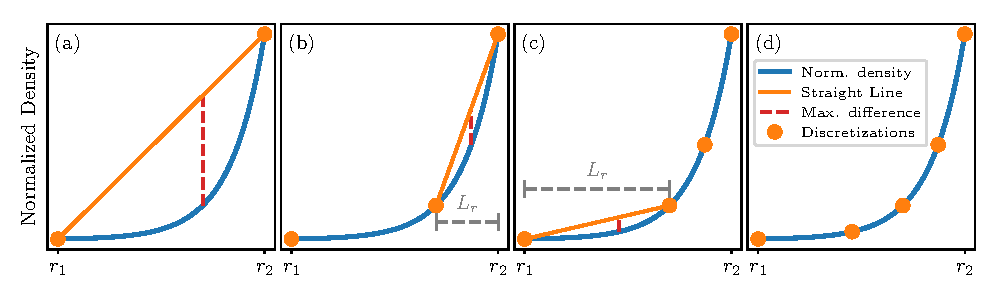
\includegraphics[width=\linewidth]{figs/tesseroids-variable-density/density-based-discretization-algorithm.pdf}
\caption{
    Ejemplo de la aplicación del algoritmo de discretización basado en densidad
    a una función densidad no lineal.
    (a)~La función densidad normalizada $\rho_n(r')$ (azul), los límites
    actuales del tesseroide (puntos naranja), y la \emph{línea recta}
    $\rho_l(r')$ (línea naranja).
    Las líneas de a trazos rojas representan la máxima diferencia de densidad
    $\Delta \rho (r')$ a la cual el tesseroide será subdividido (asumiendo que
    la desigualdad~\ref{eq:delta-density} no se satisface).
    (b)~Segunda iteración del algoritmo con una nueva \emph{línea recta}
    y máxima diferencia de densidad. El tesseroide será dividido a la
    profundidad indicada por la linea roja de a trazos.
    (c)~Tercera iteración del algoritmo.
    (d)~ Salida final del algoritmo de discretización basado en densidad,
    asumiendo que los cuatro tesseroides nuevos satisfacen la
    desigualdad~\ref{eq:delta-density}.
}
\label{fig:density-discretization-algorithm}
\end{figure}


El algoritmo puede comprenderse a través de los siguientes pasos
(Fig.~\ref{fig:density-discretization-algorithm}):

\textit{Paso 1}:
Definimos una \emph{línea recta} $\rho_l(r')$ que toma los mismos valores que
la función densidad normalizada $\rho_n(r')$ en los extremos del tesseroide
($r_1$ y $r_2$):

\begin{equation}
    \rho_l(r') =
    \frac{ \rho_n(r_2) - \rho_n(r_1) }{ r_2 - r_1 } (r' - r_1) + \rho_n(r_1).
    \label{eq:density-reference-line}
\end{equation}

\textit{Paso 2}:
Evaluamos la función de densidad normalizada y la \emph{línea recta} en un
rango de $N$ radios entre $r_1$ y $r_2$. Hemos optado por un $N = 101$, pero el
valor específico de $N$ no es crítico para el funcionamiento del algoritmo.

\textit{Paso 3}:
Calculamos la diferencia absoluta entre los valores de la \emph{línea recta}
y la función densidad normalizada:

\begin{equation}
    \Delta \rho (r') = | \rho_n(r') - \rho_l(r') |.
    \label{eq:density-abs-diff}
\end{equation}

\textit{Paso 4}:
Si la siguiente desigualdad se satisface, el tesseroide no será subdividido:

\begin{equation}
    \text{max}\{ \Delta \rho(r') \} \frac{L_r}{L_r^\text{orig}} \le \delta,
    \label{eq:delta-density}
\end{equation}

\noindent donde $L_r$ es la dimensión radial del tesseroide en consideración
(no confundir con el tesseroide \emph{original}),

\begin{equation}
    L_r = r_2 - r_1,
\end{equation}

\noindent $L_r^\text{orig}$ es la dimensión radial del tesseroide
\emph{original}, y $\delta$ es una constante positiva que denominaremos
\emph{ratio delta}.

\textit{Paso 5}:
Si la desigualdad~\ref{eq:delta-density} no se satisface, entonces dividimos el
tesseroide en dos a una profundidad dada por el radio $r_\text{max}$ a la cual
la máxima diferencia absoluta (ec.~\ref{eq:density-abs-diff}) tiene lugar.
Repetimos los pasos 1~a~5 para cada tesseroide pequeño producido por este paso.

\textit{Paso final}:
Una vez que todos los pequeños tesseroides satisfacen la
desigualdad~\ref{eq:delta-density}, cada uno es sometido al algoritmo de
discretización adaptativa bidimensional con el objeto de calcular sus efectos
gravitatorios.

En la primer iteración, la relación $L_r/L_r^\text{orig}$ es igual a 1, ya que
el tesseroide que se considera para subdividir corresponde al \emph{original}.
En las subsiguientes iteraciones, esta relación sera progresivamente menor que
1 a medida que los tesseroides son cada vez más pequeños.
La intención de este comportamiento es limitar la cantidad de divisiones a un
numero que reduzca significativamente el error numérico:
dividir un tesseroide grande con un $\text{max}\{ \Delta \rho(r') \}$ bajo
mejoraría la precisión de la integración en mayor medida que dividiendo un
tesseroide pequeño con un $\text{max}\{ \Delta \rho(r') \}$ mayor.

A mayor valor de $\delta$, se llevarán a cabo menor cantidad de divisiones,
y viceversa.
Por ende, el valor de $\delta$ controla cuántas veces los tesseroides serán
divididos basados en la función densidad, e indirectamente, determina la
precisión y el tiempo de cómputo de la integración numérica.
Surge entonces la necesidad de determinar un valor máximo de $\delta$ que
garantice una precisión aceptable mientras minimiza el tiempo de cómputo.


\subsection{Resumen del algoritmo}

En resumen, dado un tesseroide con densidad variable en profundidad según una
función continua arbitraria, proponemos seguir los siguientes pasos para
calcular numéricamente sus campos gravitatorios en cualquier punto exterior:

\textit{Paso 1:}
Aplicar el \emph{algoritmo de discretización basado en densidad} para
subdividir al tesseroide a lo largo de la dirección radial, produciendo un
conjunto de tesseroides con las mismas dimensiones longitudinales
y latitudinales que el original, pero con diferentes límites radiales.

\textit{Paso 2:}
Aplicar el \emph{algoritmo de discretización adaptativa bidimensional} a cada
tesseroide obtenido en el paso anterior.
Si es necesario, el algoritmo subdividirá cada tesseroide en las direcciones
longitudinal y latitudinal, generando un conjunto de tesseroides más pequeños.

\textit{Paso 3:}
Aplicar una \ac{GLQ} de segundo orden para calcular numéricamente los campos
gravitatorios (ec.~\ref{eq:glq-var-dens}) generados por cada tesseroide
obtenido en el paso anterior. La integración numérica incluye la función
densidad y puede ser aplicada sin modificaciones a cualquier función continua.
La suma de todos estos resultados corresponde al campo gravitatorio generado
por el tesseroide original.


\subsection{Implementación por Software}

Hemos implementado los algoritmos descriptos en las secciones anteriores
mediante el uso del lenguaje de programación Python.
El software está basado en la implementación de \citet{uieda2016} incluida en
la librería Fatiando a Terra v0.5 \citep{uieda2013}.
Los pasos que involucran un mayor tiempo de cómputo han sido escritos en
lenguaje Cython para alcanzar un mejor desempeño.
Aprovechamos la naturaleza dinámica del lenguaje Python para admitir como
parámetro de entrada funciones de densidades definidas por el usuario o la
usuaria.
Por ende, nuestro código puede ser utilizado con funciones lineales,
exponenciales, polinomiales, sinusoidales, splines cúbicas o cualquier otra
función de densidad continua sin necesidad de realizar modificaciones a su
programación.
Esta implementación se encuentra disponible libremente bajo la licencia
de código abierto BSD 3-clause.
Todo el código fuente, los scripts de Python, los datos y resultados se
encuentran disponibles a través del siguiente repositorio
\href{
    https://doi.org/10.6084/m9.figshare.8239622
}{
    doi.org/10.6084/m9.figshare.8239622
}
\citep{soler2019b} o
\href{
    https://github.com/pinga-lab/tesseroid-variable-density
}{
    github.com/pinga-lab/tesseroid-variable-density
}.
El repositorio también contiene instrucciones para replicar los resultados
presentados en este Capítulo.


%%%%%%%%%%%%%%%%%%%%%%%%%%%%%%%%%%%%%%%%%%%%%%%%%%%%%%%%%%%%%%%%%%%%%%%%%%%%%

\section{Determinación de los \emph{ratios} distancia-tamaño y \emph{delta}}

El \emph{ratio} distancia-tamaño $D$ de la discretización adaptativa y el
\emph{ratio delta} $\delta$ de la discretización basada en la densidad
determinan cuántas veces cada tesseroide será dividido y por ende controlan
indirectamente el error numérico de las integraciones.
Debemos determinar valores óptimos para $D$ y $\delta$ si deseamos asegurar
tanto una precisión numérica aceptable así como una eficiencia computacional de
los algoritmos.

\citet{uieda2016} compararon los resultados de las integraciones numéricas de
tesseroides homogéneos con las soluciones analíticas de un cascarón esférico
\citep{mikuska2006, grombein2013} con el objetivo de obtener valores
predeterminados para el \emph{ratio} distancia-tamaño $D$.
Seguiremos esta idea, pero en nuestro caso el cascarón esférico debe tener el
mismo perfil de densidad que nuestro modelo de tesseroides. \citet{lin2019}
obtuvieron la solución analítica del potencial gravitatorio generado por un
cascarón esférico con densidad lineal en la coordenada radial.
Aplicando el Teorema del Cascarón de Newton \citep{chandrasekhar1995,
binney2008}, podemos derivar expresiones para el potencial gravitatorio de un
cascarón esférico con densidades lineales, exponenciales o sinusoidales (ver
Apéndice~\ref{sec:shell}).

Con el objetivo de comparar los resultados numéricos con las soluciones
analíticas debemos construir modelos de un cascarón esférico a partir de
tesseroides.
Dividimos entonces el cascaron esférico a lo largo de las direcciones
longitudinales y latitudinales obteniendo un modelo de cascarón conformado por
$6 \times 12 = 72$ tesseroides de un tamaño de $30^\circ \times 30^\circ$.
Hemos definido varios modelos de cascarones con diferentes espesores
(Tabla~\ref{tab:shell-models}) para poder evaluar la discretización basada en
densidad en diferentes escenarios.
Los valores de espesor fueron elegidos para cubrir un amplio rango de
posibles aplicaciones: desde modelos topográficos a escalas litosféricas.
Dado que la cantidad de subdivisiones en la discretización adaptativa será
proporcional al tamaño de los tesseroides (ec.~\ref{eq:condition}),
algunas de estas configuraciones representan los peores casos.
La mayoría de las aplicaciones prácticas usarían tesseroides más pequeños que
$30^\circ \times 30^\circ \times 1000\ \text{km}$.

Las diferencias entre la solución analítica y los resultados numéricos pueden
ser calculados en un único punto de cómputo debido a la simetría rotacional del
cascarón esférico.
Sin embargo, los resultados numéricos dependen de la posición relativa entre el
punto de cómputo y el tesseroide \citep{ku1977, asgharzadeh2007, uieda2016}.
Tendremos en cuenta este fenómeno calculando dichas diferencias sobre grillas
regulares y almacenando únicamente la diferencia máxima absoluta.
Estos cálculos serán realizados sobre cuatro grillas diferentes
(Tabla~\ref{tab:grids}):
una grilla local sobre el polo, una grilla local en el ecuador, una grilla
global a altitud cero, y una grilla global a una altitud de 260km sobre la
superficie del cascarón (representando la altitud nominal del satélite GOCE).
Estas grillas cubren un amplio espectro de escenarios y asegurarán una
precisión aceptable para cada uno de ellos.

Las comparaciones entre las soluciones analíticas y los resultados numéricos
serán llevadas a cabo utilizando funciones de densidades lineales,
exponenciales y sinusoidales.
La densidad sinusoidal es incluida con el objetivo de evaluar la aproximación
numérica en sus límites de desempeño.
Repetimos estas comparaciones para cada combinación de modelos de tesseroides
en la Tabla~\ref{tab:shell-models} y grillas de la Tabla~\ref{tab:grids}.
A partir de estos resultados generalizaremos valores óptimos para $D$
y $\delta$ que garantizan errores numéricos menores a 0.1\% en comparación con
las soluciones analíticas del cascarón esférico en la mayoría de los casos.

\begin{table}
\caption{
    Descripción de los modelos de tesseroides utilizados para construir
    cascarones esféricos y caracterizar la precisión de las integraciones
    numéricas.
    El radio exterior ($R_2$) de cada modelo es igual al radio medio de la
    Tierra (6378.137 km), mientras que le radio interior ($R_1$) es determinado
    por el espesor del cascarón.
    La cantidad total y las dimensiones horizontales de los tesseroides en cada
    modelo de cascarón están detalladas según dimensiones latitudinales
    y longitudinales, respectivamente.
    \newline
}
\label{tab:shell-models}
\centering
\begin{tabular}{rccccc}
    Espesor & Tamaño de cada tesseroide  & Cantidad de tesseroides \\ \hline
    0.1 km  & $30^\circ \times 30^\circ$ & $6 \times 12 = 72$ \\
    1 km    & $30^\circ \times 30^\circ$ & $6 \times 12 = 72$ \\
    10 km   & $30^\circ \times 30^\circ$ & $6 \times 12 = 72$ \\
    100 km  & $30^\circ \times 30^\circ$ & $6 \times 12 = 72$ \\
    1000 km & $30^\circ \times 30^\circ$ & $6 \times 12 = 72$ \\
\end{tabular}
\end{table}

\begin{table}
\caption{
    Descripción de las grillas de putos de cómputo utilizadas para caracterizar
    la precisión de las integraciones numéricas.
    La altitud de las grillas es definida por encima del radio medio de la
    Tierra.
    \newline
}
\label{tab:grids}
\centering
\begin{tabular}{lccc}
    Nombre & Espaciado de la grilla & Región (grados) & Altitud (km)
    \\ \hline
    Polo      & $0.1^\circ$ &   0E /   1E / 89N / 90N & 0   \\
    Ecuador   & $0.1^\circ$ &   0E /   1E /  0N / 1N  & 0   \\
    Global    & $ 10^\circ$ & 180W / 180E / 90S / 90N & 0   \\
    Satélite  & $ 10^\circ$ & 180W / 180E / 90S / 90N & 260 \\
\end{tabular}
\end{table}


\subsection{Densidad Lineal}

El potencial gravitatorio y la componente radial del gradiente que genera un
cascarón esférico con una función de densidad lineal dada por

\begin{equation}
    \rho(r') = ar' + b,
    \label{eq:density-linear}
\end{equation}

\noindent posee soluciones analíticas dadas por las
ecuaciones~\ref{eq:shell-pot-linear} y~\ref{eq:shell-gz}. Los valores de los
coeficientes $a$ y $b$ pueden ser elegidos de forma tal que la densidad asuma
valores valores iguales a  $\rho_\text{in} = 3300$\kgpercubicm{} y
$\rho_\text{out} = 2670$\kgpercubicm{} en los radios interior ($R_\text{in}$)
y exterior ($R_\text{out}$) del cascarón, respectivamente:

\begin{equation}
    a = \frac{\rho_\text{out} - \rho_\text{in}}{R_\text{out} - R_\text{in}},
\end{equation}

\begin{equation}
    b = \rho_\text{out} -
    \frac{
        \rho_\text{out} - \rho_\text{in}
    }{
        R_\text{out} - R_\text{in}
    } R_\text{out}.
\end{equation}


\begin{figure}
\centering
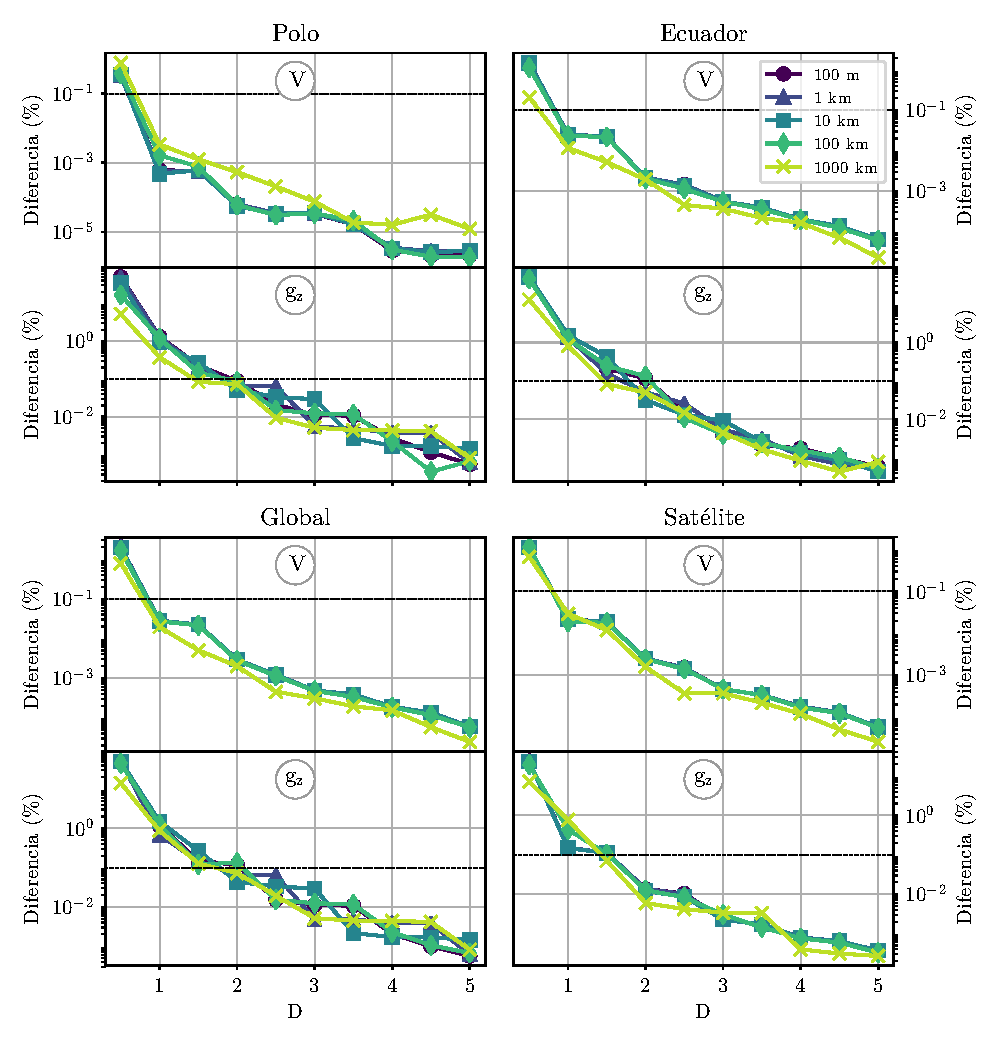
\includegraphics[width=\linewidth]{figs/tesseroids-variable-density/linear-density-diffs.pdf}
\caption{
    Diferencias entre los campos gravitatorios generados por cada modelo de
    cascarón hecho con tesseroides y sus respectivas soluciones analíticas en
    función del \emph{ratio} distancia-tamaño $D$.
    Cada modelo posee una densidad lineal (ec.~\ref{eq:density-linear}).
    Los cálculos fueron realizados sobre las cuatro grillas descriptas en la
    Tabla~\ref{tab:grids}.
    Cada curva representa la diferencia máxima absoluta entre los resultados
    numéricos y las solución analítica para un dado modelo de cascarón.
    Debido a la linealidad de la función densidad, el algoritmo de
    discretización basado en densidad no es aplicado.
    Las diferencias están reportadas como un porcentaje de las soluciones
    analíticas.
    Las líneas horizontales de a trazos y color negro representan el umbral de
    precisión de 0.1\%.
}
\label{fig:D-linear}
\end{figure}

Las diferencias absolutas definidas en la ecuación~\ref{eq:density-abs-diff}
son siempre cero para cualquier tipo de densidad lineal.
Como resultado, la desigualdad~\ref{eq:delta-density} será siempre satisfecha
y no será necesario subdividir el tesseroide en la dirección radial durante la
discretización basada en densidad.
Por lo tanto, solo la discretización adaptativa bidimensional es el único
mecanismo que controla la precisión de la integración numérica para el caso de
densidad lineal.
Por esta razón ignoraremos los valores de $\delta$ y solo determinaremos el
mínimo valor de $D$ necesario para garantizar una precisión aceptable.

Calculamos el potencial gravitatorio ($V$) y su derivada vertical ($g_z$)
para cada modelo de cascarón esférico definido en la
Tabla~\ref{tab:shell-models} en cada grilla de cómputo de la
Tabla~\ref{tab:grids}.
Las derivadas horizontales del potencial son iguales a cero fuera del cascarón
debido a la simetría rotacional, y por ende son omitidos del análisis.
Estos cálculos son repetidos para valores de \emph{ratio} distancia-tamaño $D$
desde 0.5 a 5 con incrementos de 0.5.
Luego calculamos la diferencia absoluta entre los resultados numéricos y las
soluciones analíticas para el cascarón.
La Figura~\ref{fig:D-linear} muestra la máxima diferencia absoluta para cada
modelo de cascarón y grilla de cómputo como función de $D$.
Las diferencias se muestran relativas a la solución analítica para cada
cascarón.
Finalmente, seleccionamos el valor óptimo de $D$ como el menor valor para el
cual la diferencia es menor a 0.1\%.

A partir de la Figura~\ref{fig:D-linear} podemos observar que los errores
relativos para el potencial $V$ y para su derivada vertical $g_z$ caen por
debajo del umbral de 0.1\% para valores de $D=1$ y $D=2.5$, respectivamente.
Notablemente, un valor de $D=2$ sería suficiente para $g_z$ en el caso de una
grilla a altitud satelital.
Para el resto de las configuraciones, dichos valores son consistentes
e independientes del espesor de cascarón o de la ubicación geográfica.


\subsection{Densidad exponencial}

Para una función de densidad exponencial, la discretización basada en densidad
será aplicada con anterioridad al algoritmo de discretización adaptativa.
Esto significa que los valores óptimos para el \emph{ratio} distancia-tamaño
$D$ y el \emph{ratio delta} $\delta$ (ec.~\ref{eq:delta-density}) deben ser
determinados simultáneamente.
Para ello llevamos a cabo un análisis de error similar al que aplicamos en el
caso de densidad lineal.
Ahora el cascarón esférico poseerá una densidad según una función exponencial
que asume los valores de $\rho_\text{out} = 2670$\kgpercubicm{}
y $\rho_\text{in} = 3300$\kgpercubicm{} en las superficies externas
e internas, respectivamente, y que se define de la siguiente manera:

\begin{equation}
    \rho(r') = A e^{- b \frac{r' - R_1}{R_2 - R_1}} + C,
    \label{eq:density-exp}
\end{equation}

\noindent donde

\begin{equation}
    A = \frac{\rho_\text{in} - \rho_\text{out}}{1 - e^{-b}},
\end{equation}

\begin{equation}
    C = \rho_\text{in} - A,
\end{equation}

\noindent y $b$ es una constante adimensional que determina el grado de
variabilidad de la función. Un valor mayor de $b$ aumenta la máxima pendiente
de la función densidad (Fig.~\ref{fig:exp-densities}).

\begin{figure}
\centering
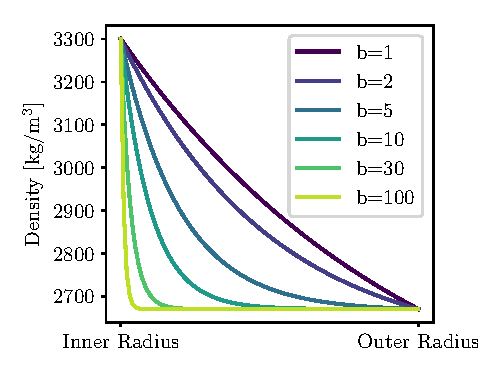
\includegraphics[width=0.5\linewidth]{figs/tesseroids-variable-density/exponential-densities.pdf}
\caption{
    Funciones de densidad exponencial asignadas a los modelos de cascarón
    esférico para la determinación del \emph{ratio} $\delta$.
    Cada función densidad corresponde a diferentes valores de $b$ en la
    ecuación~\ref{eq:density-exp}.
}
\label{fig:exp-densities}
\end{figure}


\subsubsection{Exploración del espacio $D$-$\delta$}

Nuestro objetivo es hallar una combinación de valores para $D$ y $\delta$ que
produzcan un error numérico menor al umbral de 0.1\% mientras minimicen el
tiempo de cómputo.
Para ello hacemos uso del método de búsqueda en grilla (\emph{grid search} en
inglés) y calculamos el error numérico para cada par ($D$, $\delta$)
perteneciente a una grilla en el espacio $D$-$\delta$
(Fig.~\ref{fig:grid-search}).
Con el objeto de obtener un óptimo desempeño del algoritmo, buscamos el par
($D$, $\delta$) que minimice el número de subdivisiones de tesseroides mientras
mantengan el error numérico por debajo del umbral de 0.1\%.
Este requisito se traduce en minimizar el valor de $D$ y maximizar el valor de
$\delta$.

Dado que la búsqueda en grilla es un proceso computacionalmente costoso,
limitamos el análisis a un valor alto de $b=30$ (Fig.\ref{fig:exp-densities})
y la grilla de cómputo \emph{Global} definida en la Tabla~\ref{tab:grids}.
Calculamos la diferencia relativa entre el resultado numérico y la solución
analítica del potencial gravitatorio ($V$) y su derivada vertical ($g_z$) para
cada modelo de cascarón definido en la Tabla~\ref{tab:shell-models}.
La Figura~\ref{fig:grid-search} muestra la máxima diferencia obtenida para
todos los modelos de cascarón.
Las líneas de a trazos representan un contorno correspondiente al 0.1\% de
error relativo, por ende los puntos interiores a ella son los que caen debajo
de dicho umbral.
Además, la figura destaca los valores de $D$ obtenidos en la Sección anterior
para el caso de densidad lineal ($D_\text{linear}$).

Los valores más chicos de $D$ que se encuentran debajo del umbral de 0.1\%
coinciden con los valores $D_\text{linear}$ tanto para $V$ como para $g_z$.
Estos resultados indican que los valores de $D_\text{linear}$ obtenidos pueden
ser extrapolados a los casos de densidades no lineales.
Esto no es una sorpresa, ya que la discretización adaptativa bidimensional y la
discretización basada en densidad son independientes una de la otra: la primera
divide al tesseroide en las direcciones horizontales, mientras que la otra lo
hace solo en la dirección radial.
Por ende, es de esperar que el valor óptimo de $\delta$ sea independiente del
valor óptimo de $D$.
Dado que la búsqueda en grilla fue limitada a una grilla de cómputo específica
y a un único valor de $b$, en los próximos párrafos realizaremos un análisis
más detallado para determinar un valor óptimo de $\delta$ para el caso de
densidad exponencial.

\begin{figure}
\centering
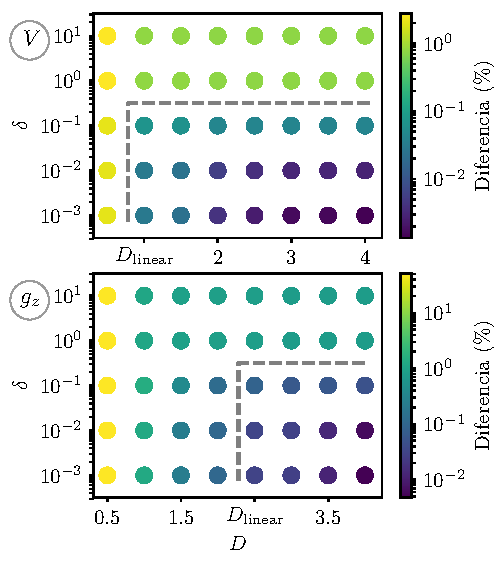
\includegraphics[width=0.5\linewidth]{figs/tesseroids-variable-density/grid-search.pdf}
\caption{
    Exploración del error numérico en el espacio $D$-$\delta$.
    Los valores porcentuales de diferencia fueron obtenidos a partir de la
    comparación entre las soluciones analíticas y las aproximaciones numéricas
    de los campos gravitatorios ($V$ y $g_z$) generados por un cascarón
    esférico con una densidad exponencial
    (ec.~\ref{eq:density-exp}) con $b=30$.
    Estas comparaciones fueron realizadas sobre la grilla de cómputo
    \emph{Global} (Tabla~\ref{tab:grids}), con los modelos de cascarón
    esféricos detallados en la Tabla~\ref{tab:shell-models}.
    Los valores de diferencias porcentuales fueron obtenidos como la máxima
    diferencia de entre todos los modelos de cascarón.
    Los puntos interiores a la región delimitada por las lineas de a trazos son
    los que presentan un error por debajo del umbral de 0.1\%.
    Los valores de $D$ obtenidos para el caso de densidad lineal para cada
    campo gravitatorio se encuentran identificados con $D_\text{linear}$.
    }
\label{fig:grid-search}
\end{figure}


\subsubsection{Determinación del \emph{ratio delta}}

Habiendo fijado valores de $D$ iguales a los obtenidos para el caso de
densidad lineal, nos encontramos en condiciones de explorar los errores de
integración como función de $\delta$ en mayor detalle.
Calcularemos la diferencia entre el error numérico y las soluciones analíticas
para todas las combinaciones de grillas de cómputo (Tabla~\ref{tab:grids})
y modelos de cascarón esférico (Tabla~\ref{tab:shell-models}),
variando los valores de $\delta$ entre $10^{-3}$ y $10^{1}$.
Los cálculos son repetidos para cada valor de $b \in \{1, 2, 5, 10, 30, 100\}$
(Fig.~\ref{fig:exp-densities}) con el objeto de analizar la precisión del
método para diversos tipos de funciones exponenciales.
Dado que valores mayores de $\delta$ producen menores subdivisiones, nuestra
intención es hallar los valores máximos de $\delta$ que producen una diferencia
relativa por debajo del umbral de 0.1\%.
La Figura~\ref{fig:delta-exponential} muestra las diferencias relativas
resultantes para $V$ y $g_z$ como función de $\delta$.
Por brevedad, cada curva corresponde a la diferencia máxima entre todos los
modelos de cascarón esférico.
Las curvas correspondientes a $b=1$ y $b=2$ se encuentran por debajo del umbral
0.1\% para todos los valores de $\delta$ y no se ven modificadas para valores
de $\delta > 0.8$, indicando que esas funciones de densidad son los
suficientemente suaves como para poder prescindir de discretizaciones en la
dirección radial.
Para todos los otros valores de $b$, las diferencias caen debajo del umbral si
$\delta=0.1$.
Estos resultados indican que no hay una relación significativa entre la
suavidad de la densidad exponencial y el error numérico.

\begin{figure}
\centering
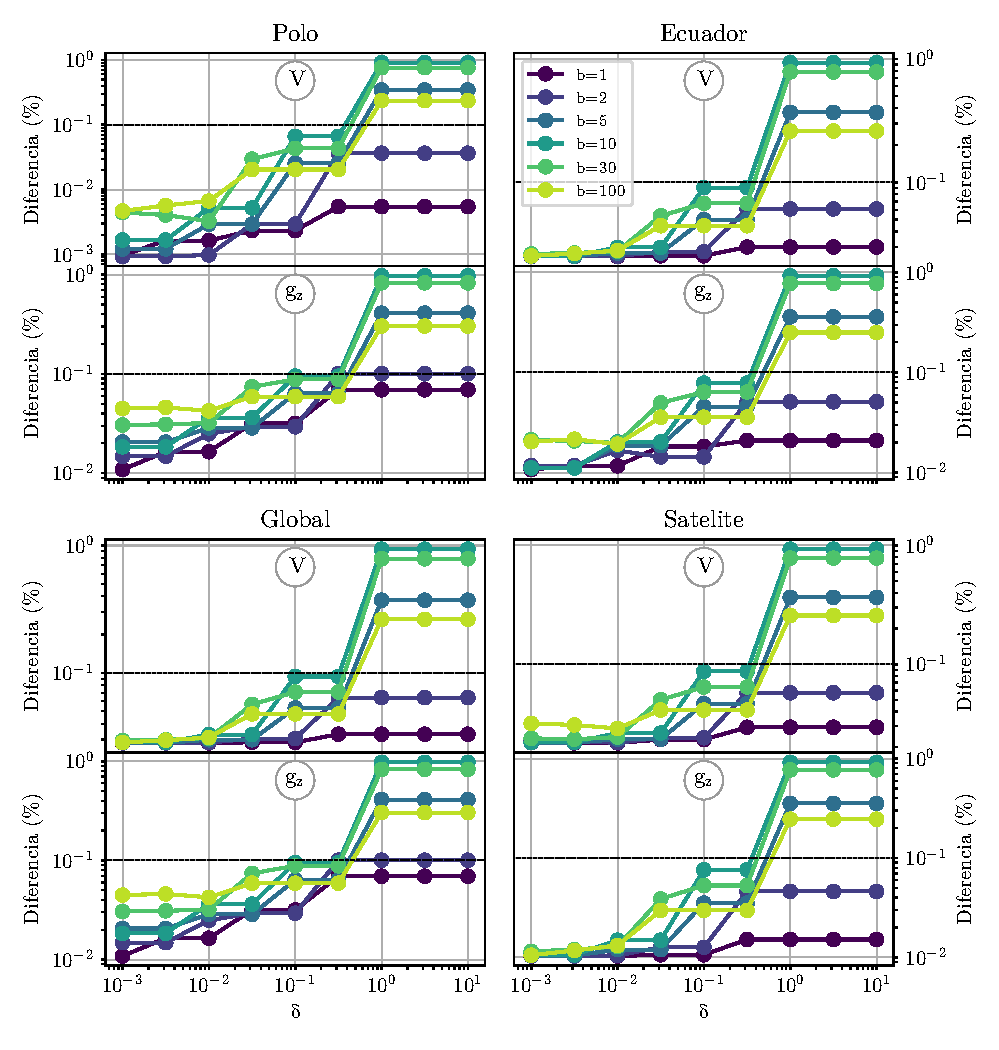
\includegraphics[width=\linewidth]{figs/tesseroids-variable-density/exponential-density-diffs.pdf}
\caption{
    Diferencias entre el error numérico y las soluciones analíticas como
    función del \emph{ratio} $\delta$ para varias funciones de densidad
    exponenciales.
    Estas comparaciones fueron llevadas a cabo para cada combinación entre los
    modelos de cascarón (Tabla~\ref{tab:shell-models}) y las grillas de cómputo
    (Tabla~\ref{tab:grids}) haciendo uso de un valor fijo de $D$. Cada curva
    corresponde a la diferencia máxima obtenida para cada modelo de cascarón
    para un valor particular de $b$ (ec.~\ref{eq:density-exp}). Las diferencias
    están reportadas como un porcentaje de las soluciones analíticas. Las
    líneas horizontales de a trazos y color negro representan el umbral de
    precisión de 0.1\%.
    }
\label{fig:delta-exponential}
\end{figure}


\subsection{Densidad sinusoidal}

Hasta ahora hemos analizado el comportamiento de la discretización basada en
densidad contra funciones de densidades lineales y exponenciales.
Sin embargo, este nuevo algoritmo es adecuado para ser utilizado con funciones
continuas más complejas, por ejemplo funciones no monotónicas o que presenten
múltiples puntos de inflexión.
Aunque este tipo de funciones de densidad son cuanto mucho raras de encontrar
en seteos geológicos, queremos someter nuestro algoritmo a estos casos con el
objetivo de mostrar su capacidad para resolver situaciones más complejas que
funciones lineales y exponenciales.
Además, obtener un valor óptimo del \emph{ratio} $\delta$ para casos de
funciones de densidades irreales nos permitiría extrapolarlo a casos más
simples y realistas.
Es por esta razón que los análisis que se describirán a continuación están
destinados a someter el algoritmo a sus extremos y no para emular un escenario
real.

Consideremos modelos de cascarones específicos con una función de densidad
sinusoidal que se define de la siguiente manera:

\begin{equation}
    \rho(r') = A \sin \left( 2 \pi b \frac{r' - R}{R_2 - R_1} \right) + A,
    \label{eq:density-sine}
\end{equation}

\noindent donde $A$ es una constante que controla la amplitud y la traslación
vertical de la función seno, $R$ es el radio medio de la Tierra y $b$ es una
constante adimensional que regula cuántos períodos de la función trigonométrica
serán incluidos dentro de los radios interior y exterior.
La solución analítica para el potencial $V$ y su gradiente vertical $g_z$ que
genera un cascarón esférico con una densidad sinusoidal puede hallarse en el
Apéndice~\ref{sec:shell}.

Calculamos la diferencia relativa entre los resultados numéricos y la solución
analítica para $V$ y $g_z$ para cada combinación de modelos de cascarones
(Tabla~\ref{tab:shell-models}) y grillas de cómputo (Tabla~\ref{tab:grids}).
Hemos fijado el \emph{ratio} distancia-tamaño $D$ a los valores obtenidos para
el caso de densidad lineal y exploramos valores de $\delta$ entre $10^{-4}$
y $1$.
Los cálculos fueron repetidos para valores de $b$ iguales a 1, 2, 5 y 10.
(Fig.~\ref{fig:sine-densities}). En todos los casos el valor de $A$ fue fijado
a 1650\kgpercubicm{}.

\begin{figure}
\centering
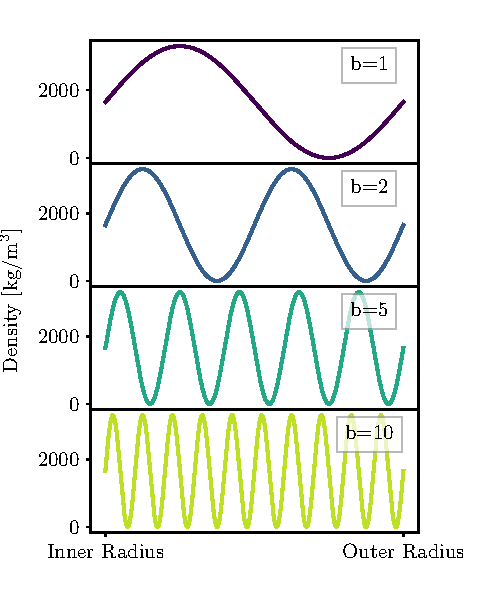
\includegraphics[width=0.5\linewidth]{figs/tesseroids-variable-density/sine-densities.pdf}
\caption{
    Densidades sinusoidales asignadas a los cascarones esféricos durante la
    determinación del \emph{ratio} $\delta$.
    Cada función de densidad corresponde a un valor distinto de $b$ en la
    ecuación~\ref{eq:density-sine}.
}
\label{fig:sine-densities}
\end{figure}

\begin{figure}
\centering
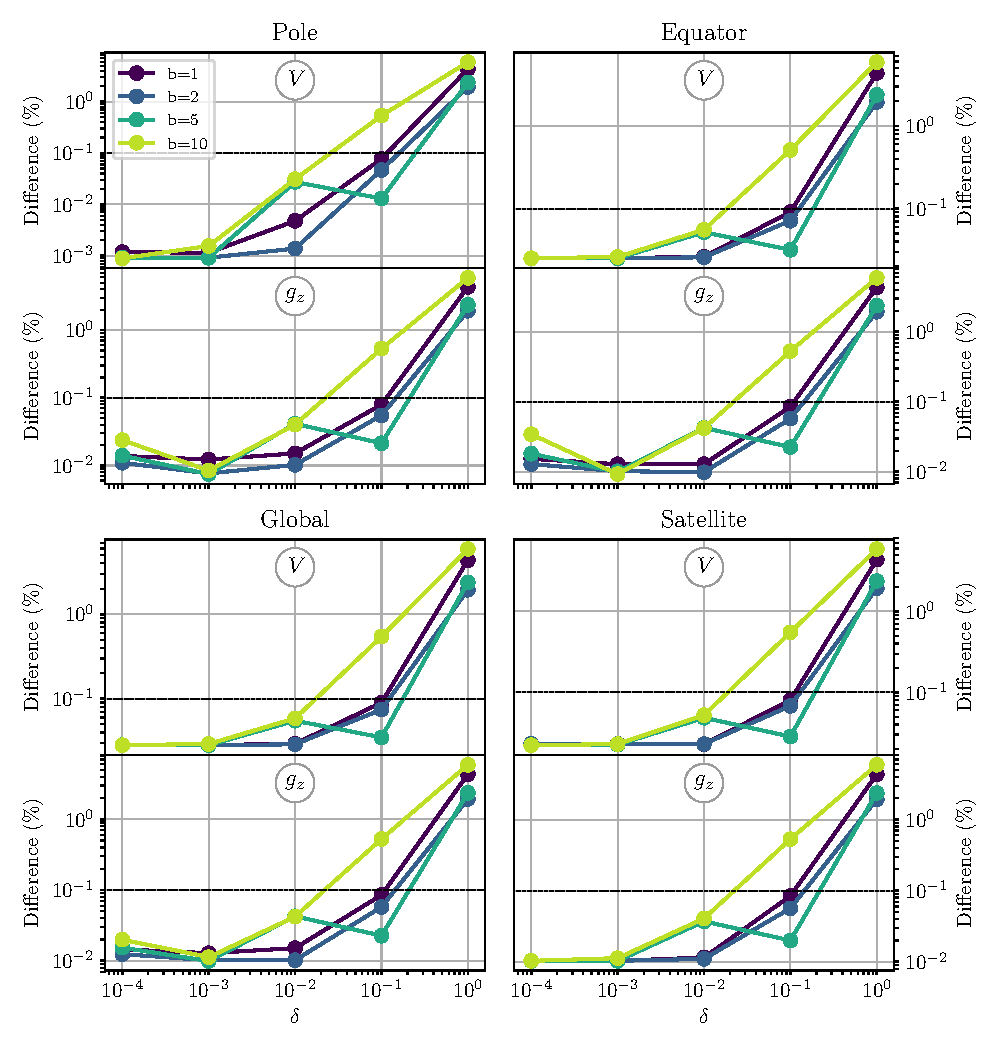
\includegraphics[width=\linewidth]{figs/tesseroids-variable-density/sine-density-diffs.pdf}
\caption{
    Diferencias entre los resultados numéricos y las soluciones analíticas como
    función de $\delta$ para diferentes funciones de densidad sinusoidales.
    Las comparaciones fueron llevadas a cabo para cada modelo de cascarón
    (Tabla~\ref{tab:shell-models}) y cada grilla de cómputo
    (Tabla~\ref{tab:grids}) haciendo uso de un valor fijo de $D$.
    Cada curva corresponde a la diferencia máxima obtenida para cada modelo de
    cascarón para un valor particular de $b$ (ec.~\ref{eq:density-sine}).
    Las diferencias están reportadas como un porcentaje de las soluciones
    analíticas. Las líneas horizontales de a trazos y color negro representan
    el umbral de precisión de 0.1\%.
    }
\label{fig:delta-sine}
\end{figure}

La Figura~\ref{fig:delta-sine}
muestra las diferencias relativas entre los resultados numéricos y las
soluciones analíticas para casos de densidades sinusoidales.
Nuevamente, cada curva corresponde a la diferencia máxima para cada modelo de
cascarón.
Para todos los valores de $b$, a excepción de $b=10$, las diferencias caen
debajo del umbral 0.1\% para $\delta = 0.1$.
En el caso de $b=10$, un menor valor de $\delta = 0.01$ es necesario para
alcanzar dicho umbral.
Vale notar que incluso para el caso de $b=10$, las diferencias obtenidas
utilizando $\delta = 0.1$ se encuentran debajo del 1\%.


%%%%%%%%%%%%%%%%%%%%%%%%%%%%%%%%%%%%%%%%%%%%%%%%%%%%%%%%%%%%%%%%%%%%%%%%%%%%%%%

\section{Desempeño del algoritmo}

Dado que el algoritmo de discretización basada en densidad introduce
subdivisiones a lo largo de la dirección radial, es razonable suponer que el
tiempo de cómputo para el caso de densidades variables será más alto que en el
caso de densidades homogéneas.
Comparar directamente el tiempo de cómputo en ambos casos no podría ser
realizado de forma significativa, ya que dependería fuertemente en la
implementación del algoritmo, la elección del lenguaje de programación y la
función densidad en particular.
Con el objetivo de obtener un indicador sobre cuánto aumenta el costo
computacional, elegimos la cantidad de subdivisiones al tesseroides en la
discretización basada en densidad como una variable \emph{proxy}.

Analizamos densidades exponenciales (ec.~\ref{eq:density-exp}) con valores de
$b$ iguales a 1, 2, 5, 10, 30 y 100, y densidades sinusoidales
(ec.~\ref{eq:density-sine}) con valores de $b$ iguales a 1, 2, 5, y 10.
Aplicamos el algoritmo de discretización basado en densidad sobre cada una de
esas funciones y registramos la cantidad de divisiones que produce en cada
caso.
Las Figuras~\ref{fig:number-of-tesseroids}a y~\ref{fig:number-of-tesseroids}b
muestran las densidades exponenciales y sinusoidales junto con sus
correspondientes puntos de discretización como círculos naranja.

En el caso de densidad exponencial, el algoritmo realiza una única subdivisión
independientemente del valor de $b$.
Por lo tanto, el tiempo de cómputo podría estimarse como el doble del caso de
una densidad homogénea (asumiendo implementaciones idénticas).
Por otro lado, la Figura~\ref{fig:number-of-tesseroids}c muestra una relación
casi lineal entre el número de divisiones para el caso de densidad sinusoidal
y los valores de $b$.
Por lo tanto, el tiempo de cómputo en estos casos parece depender de la
cantidad de períodos de la función sinusoidal contenidos dentro de los límites
del tesseroide.

\begin{figure}
\centering
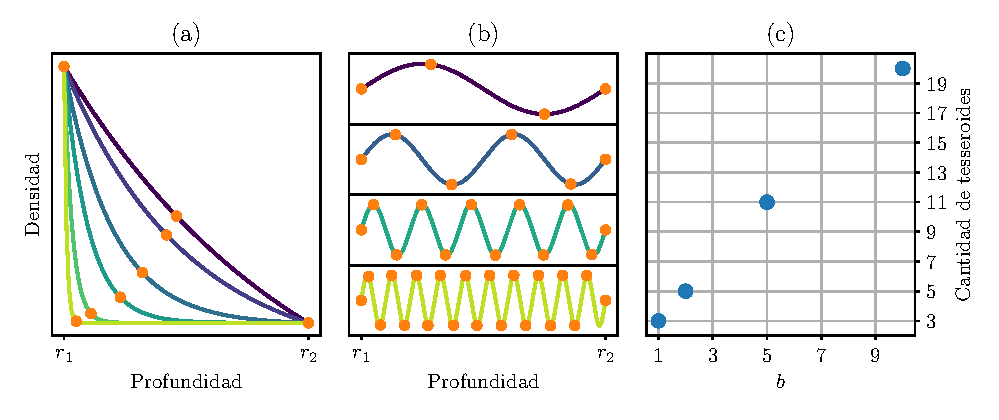
\includegraphics[width=\linewidth]{figs/tesseroids-variable-density/number-of-tesseroids.pdf}
\caption{
    Cantidad de subdivisiones realizadas por el algoritmo de discretización
    basada en densidad (con $\delta = 0.1$) en caso de
    (a)~funciones de densidad exponencial con los mismos valores de $b$
    presentes en la Fig.~\ref{fig:exp-densities},
    (b)~funciones de densidad sinusoidal con los mismos valores de $b$
    presentes en la Fig.~\ref{fig:sine-densities}.
    En ambas figuras, las ubicaciones de las discretizaciones están marcadas
    con círculos naranja.
    (c)~Muestra la cantidad de tesseroides obtenidos en el caso de densidad
    sinusoidal como función de $b$.
}
\label{fig:number-of-tesseroids}
\end{figure}


%%%%%%%%%%%%%%%%%%%%%%%%%%%%%%%%%%%%%%%%%%%%%%%%%%%%%%%%%%%%%%%%%%%%%%%%%%%%%%%

\section{Aplicación a la Cuenca Neuquina}

Hemos aplicado los nuevos algoritmos y los valores óptimos para $D$
y $\delta$ determinados previamente para calcular los efectos gravitatorios de
la Cuenca Neuquina, una cuenca sedimentaria localizada al este de los Andes,
entre las latitudes 32$^\circ$S y 40$^\circ$S (Fig.~\ref{fig:neuquen-basin}a).
La cuenca incluye siliciclástos marinos y sedimentarios, carbonatos
y evaporitas acumuladas durante el Jurásico y el Cretácito constituyendo un
registro estratigráfico hasta 5000m de profundidad \citep{howell2005}.

\begin{figure}
\centering
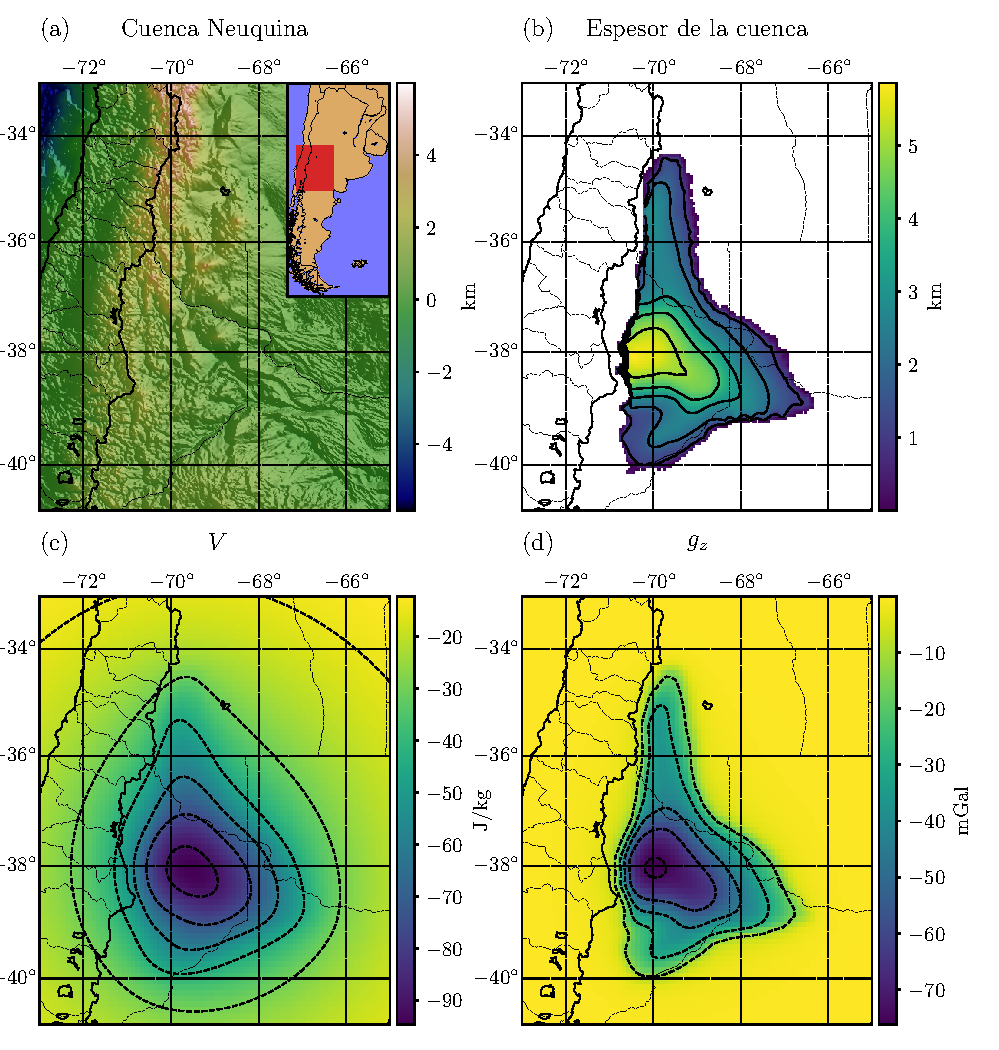
\includegraphics[width=\linewidth]{figs/tesseroids-variable-density/neuquen-basin.pdf}
\caption{
    Efectos gravitatorios de la Cuenca Neuquina modelada utilizando tesseroides
    con una densidad exponencial como función de la profundidad.
    (a)~Topografía de la Cuenca Neuquina (en km) y su ubicación geográfica en
    Sudamérica,
    (b)~espesor de la cuenca sedimentaria \citep[en metros;][]{heine2007}
    (c)~potencial gravitatorio resultante $V$,
    (d)~componente vertical del gradiente ($g_z$),
    calculadas a 10km de altitud sobre el radio medio de la Tierra.
}
\label{fig:neuquen-basin}
\end{figure}

\begin{figure}
\centering
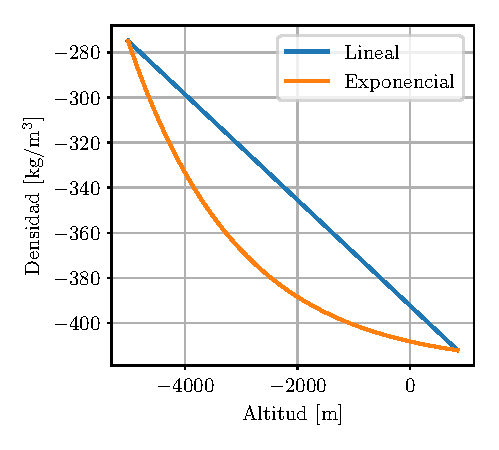
\includegraphics[width=0.5\linewidth]{figs/tesseroids-variable-density/neuquen-basin-densities.pdf}
\caption{
    Densidades lineales y exponenciales utilizadas para el cálculo de los
    campos gravitacionales generados por un modelo de la Cuenca Neuquina
    compuesto por tesseroides.
    La altitud se define por encima del radio medio de la Tierra, y sus eje se
    extiende entre el puntos más profundo hasta el punto más alto de la cuenca.
}
\label{fig:neuquen-basin-densities}
\end{figure}


\begin{figure}
\centering
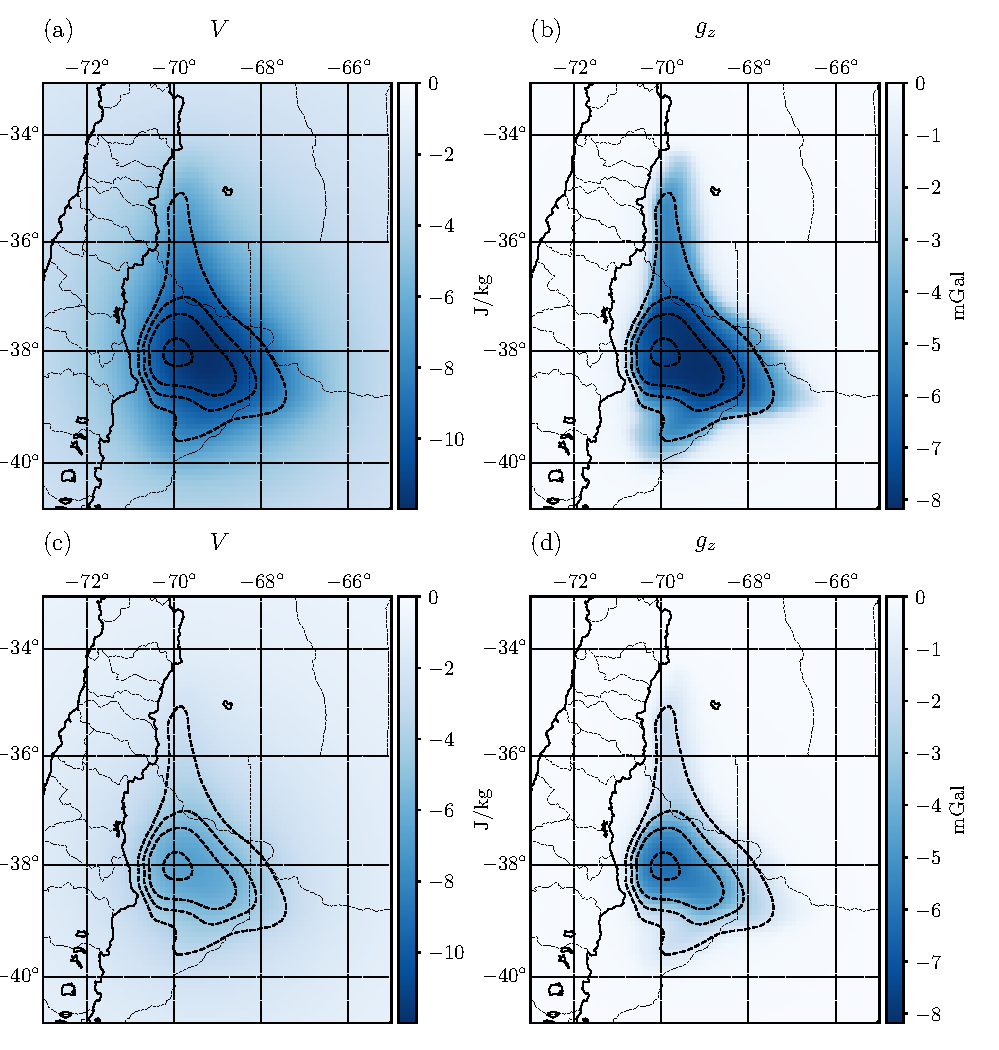
\includegraphics[width=\linewidth]{figs/tesseroids-variable-density/neuquen-basin-diffs.pdf}
\caption{
    Diferencias entre los campos gravitatorios generados por el modelo de
    tesseroides de la Cuenca Neuquina con una densidad exponencial y con el
    mismo modelo pero con densidades homogéneas y lineales.
    \mbox{(a)-(b)}~Diferencias de $V$ y $g_z$ entre el modelo con densidad
    exponencial y el modelo con densidad homogénea,
    \mbox{(c)-(f)}~diferencias de $V$ y $g_z$ entre el modelo con densidad
    exponencial y el modelo con densidad lineal,
    calculadas a 10km de altitud sobre el radio medio de la Tierra.
}
\label{fig:neuquen-basin-diffs}
\end{figure}

El espesor del paquete sedimentario fue digitalizado a partir de
\citet{heine2007} sobre una grilla regular con una resolución de 0.05$^\circ$
en las direcciones longitudinal y latitudinal (Fig.~\ref{fig:neuquen-basin}b).
Creamos un modelo del paquete sedimentario a partir de tesseroides de
$0.05^\circ \times 0.05^\circ$ ubicados sobre cada nodo de la grilla.
El límite superior de cada tesseroide fue fijado a al altitud media de la
topografía de la cuenca (845\m{} sobre el radio medio de la Tierra) y el límite
inferior es seleccionado de forma tal que cada tesseroide posea la misma
dimensión que el espesor de la cuenca sobre el correspondiente punto de la
grilla.

Además debemos definir una función densidad para el modelo de tesseroides.
\citet{sigismondi2012} determinó valores mínimos y máximos para el contraste de
densidad de la Cuenca Neuquina de -412\kgpercubicm{} y -275\kgpercubicm{},
respectivamente.
Hemos elegido una variación de densidad exponencial (ec.~\ref{eq:density-exp})
que asume el valor mínimo en la superficie superior y un valor máximo a una
profundidad de 5014\m{} (la región más profunda de la cuenca), con un valor de
$b$ igual a 3.
Esta variación de densidad se encuentra dentro de los ordenes de magnitud
utilizados por \citet{cowie1990} y \citet{cordell1973}.
La función de densidad se muestra en la
Figura~\ref{fig:neuquen-basin-densities}.

Finalmente, hemos calculado el potencial gravitatorio $V$ y la componente
vertical de su gradiente ($g_z$) sobre una grilla de cómputo compuesta por
$159\times163$ nodos (un espaciado de $0.05^\circ$ en las direcciones
longitudinal y latitudinal) a una altitud de 10\km{} sobre el radio medio de la
Tierra.
Los campos resultantes pueden apreciarse en las
Figuras~\ref{fig:neuquen-basin}c-d.

Calculamos las diferencias entre los resultados para la densidad exponencial
y para aquellos generados por el mismo modelo pero con una densidad constante
dada por el valor medio entre -412\kgpercubicm{} y -275\kgpercubicm{}.
Además calculamos las diferencias entre el modelo de densidad exponencial y uno
con densidad lineal que asume estos dos valores en los puntos más altos y más
profundos de la cuenca (Fig.~\ref{fig:neuquen-basin-densities}).
Las Figuras~\ref{fig:neuquen-basin-diffs}a-b
y ~\ref{fig:neuquen-basin-diffs}c-d muestran las diferencias con las densidad
constante y con la densidad lineal, respectivamente.
La diferencia máxima absoluta en los campos $g_z$ es aproximadamente de
8\mGal{} para el caso de densidad homogénea y aproximadamente de 6\mGal{} para
el caso lineal.
Estas discrepancias se encuentra bien por encima de los errores de la mayoría
de los relevamientos gravimétricos.


%%%%%%%%%%%%%%%%%%%%%%%%%%%%%%%%%%%%%%%%%%%%%%%%%%%%%%%%%%%%%%%%%%%%%%%%%%%%%%%

\section{Discusión}

Al incluir la función densidad dentro de la \ac{GLQ}, el método aquí descripto
puede ser aplicado sin ninguna modificación a cualquier tesseroide cuya
densidad puede representarse por una función continua en la dirección radial.
El algoritmo de discretización basado en la densidad divide el tesseroide a lo
largo de la dirección radial con el objetivo de garantizar una precisa
integración.
Este algoritmo es independiente de la integración \ac{GLQ} y puede
potencialmente ser aplicado para determinar una óptima discretización a la hora
de aproximar una función mediante funciones lineales de a pasos \citep{lin2019}
o funciones polinomiales de a pasos \citep{fukushima2018}.

Nuestros resultados experimentales muestran que la discretización adaptativa
bidimensional es suficiente para alcanzar errores debajo del 0.1\% en conjunto
con una \ac{GLQ} de segundo orden en caso de densidades lineales
(Fig.~\ref{fig:D-linear}).
Los valores del \emph{ratio} distancia-tamaño determinados para el potencial
gravitatorio ($D=1$) y para su derivada vertical ($D=2.5$) son compatibles por
los valores determinados por \citet{uieda2016}.
Estos resultados muestran además que no existe una relación significativa entre
la precisión del método y el espesor del modelo de tesseroides.

La exploración del espacio $D$-$\delta$ para el caso de una densidad
exponencial (Fig.~\ref{fig:grid-search}) muestra que los valores de $D$
determinados para el caso lineal son igualmente válidos para ser aplicados al
caso exponencial.
Además, las diferencias con respecto a las soluciones analíticas caen por
debajo del umbral de 0.1\% solo para valores de $\delta$ menores a 0.1.
Por lo tanto, la aplicación de la discretización basada en la densidad es
necesaria para alcanzar el nivel de precisión deseada en casos de
densidades no lineales.

Un análisis de errores más detallados muestra que el valor de $\delta = 0.1$ es
suficiente para garantizar errores por debajo del 0.1\% para cualquiera de las
funciones exponenciales (Fig.~\ref{fig:delta-exponential}) y para la mayoría de
las funciones sinusoidales (Fig.~\ref{fig:delta-sine}) que aquí se han probado.
La excepción se presenta en el caso de una función sinusoidal con $b = 10$
(ec.~\ref{eq:density-sine}),
para la cual un valor de $\delta = 0.01$ es necesario para alcanzar el umbral
0.1\%.
Sin embargo, utilizar un valor de $\delta = 0.1$ en este caso produce
resultados con errores por debajo del 1\%.

Aunque los algoritmos aquí propuestos pueden ser aplicados a cualquier función
de densidad continua, los valores óptimos de $D$ y $\delta$ fueron
empíricamente determinados solo para funciones lineales, exponenciales
y sinusoidales.
Por lo tanto, solo podemos afirmar con certeza que estos valores producen
resultados con errores por debajo de 0.1\% para los tipos de funciones
nombradas.
Sin embargo, todas las experiencias numéricas incluyen los escenarios menos
favorables (puntos de cómputo sobre la superficie de los tesseroides,
tesseroides de gran tamaño, funciones densidad altamente variables, etc.).
Por esta razón, es plausible extrapolar los valores óptimos de $D$ y $\delta$
a cualquier densidad continua que represente variaciones realistas de
estructuras geológicas.
A pesar de esto, alentamos a los usuarios y las usuarias de estos algoritmos
a llevar a cabo experimentaciones similares con el objetivo de evaluar su
precisión en caso de utilizar funciones de densidades más complejas que las
aquí probadas.

El análisis del desempeño del algoritmo muestra que el tiempo de cómputo
en los casos de densidades no lineales es como mínimo el doble del
necesario para el caso de densidad homogénea o lineal.
Esta proporcionalidad puede aumentar con la cantidad de puntos de inflexión de
la función densidad.
Como en la mayoría de los métodos numéricos, existe un compromiso entre tiempo
de cómputo y precisión.
Sin embargo, los perfiles de densidad suelen tener pocos puntos de inflexión en
la mayoría de las aplicaciones geofísicas.
Por lo tanto, el tiempo de cómputo se encontrará en el mismo orden de magnitud
que el caso de densidad homogénea para la mayoría de las aplicaciones en el
mundo real.

%%%%%%%%%%%%%%%%%%%%%%%%%%%%%%%%%%%%%%%%%%%%%%%%%%%%%%%%%%%%%%%%%%%%%%%%%%%%%%%

\section{Conclusiones}

Hemos desarrollado una nueva metodología para calcular el potencial
gravitatorio y su gradiente generados por un tesseroide con una densidad dada
por una función continua de la coordenada radial.
Este método resuelve numéricamente integrales volumétricas mediante la
\ac{GLQ} incluyendo la función densidad dentro del integrando.
Mediante una implementación del mismo en lenguaje Python, los usuarios
y las usuarias pueden definir su propia función densidad y servirla como
entrada al algoritmo.
Esto permite el uso de funciones continuas arbitrarias sin necesidad de
realizar modificaciones sobre el método o el software.
La precisión de la integración numérica es controlada automáticamente por un
algoritmo de discretización adaptativa bidimensional y un nuevo algoritmo de
discretización basado en densidad.
El primero subdivide iterativamente al tesseroide en caso de que las relaciones
entre la distancia al punto de cómputo y las dimensiones longitudinal
y latitudinal del tesseroide sean menores que un \emph{ratio} distancia-tamaño
$D$ predefinido.
Este algoritmo minimiza los errores de integración a cuando el punto de
cómputo se encuentra cerca del tesseroide.
Sin embargo, la discretización adaptativa por sí sola no es suficiente para
garantizar una precisión aceptable en caso de tesseroides con densidades no
lineales.
Para solucionar esto, el algoritmo de discretización basada en densidad divide
al tesseroide a lo largo de la dirección radial en los lugares donde la
\emph{máxima variación} de la función densidad ocurre.
La cantidad de subdivisiones a lo largo del radio, y por ende la precisión del
cómputo, están controladas por el parámetro \emph{delta} $\delta$.
Este nuevo algoritmo está diseñado para minimizar el error debido a la
incapacidad de la \ac{GLQ} de producir aproximaciones precisas en caso de
funciones de densidad con variaciones pronunciadas.

Hemos determinado de manera empírica valores óptimos para los parámetros $D$
y $\delta$ comparando los resultados numéricos con soluciones analíticas para
cascarones esféricos.
Nuestro análisis incluye un rango de modelos de tesseroides y grillas de
cómputo así como funciones de densidades de las más utilizadas en problemas
reales.
Estos valores minimizan el tiempo de cómputo mientras mantienen el error
numérico por debajo de un umbral de 0.1\%.
Las funciones de densidad utilizadas para establecer estos valores óptimos
fueron lineales, exponenciales y sinusoidales.
La función lineal representa la variación más sencilla de densidad y no
requiere la aplicación de una discretización basada en densidad.
Mediante este análisis hemos obtenido valores óptimos para el \emph{ratio}
distancia-tamaño $D$ de 1 y 2.5 para el potencial gravitatorio y para su
gradiente, respectivamente.
Con el objetivo de analizar la precisión de la discretización basada en
densidad, hemos calculado el error numérico para casos de densidades
exponenciales, desde funciones suaves hasta funciones con fuertes pendientes,
e incluso para funciones sinusoidales de diferentes longitudes de onda.
Vale notar que la densidad sinusoidal fue tomada en cuenta con la intención de
someter al algoritmo a sus extremos y no para emular escenarios de la vida
real.
Valores de $\delta$ iguales a 0.1 son suficientes para garantizar errores
numéricos por debajo del umbral de 0.1\% para la mayoría de los casos
examinados.
Estos resultados podrían ser extrapolados a otras funciones continuas de
densidad que sean lo suficientemente suaves. Tal y como es el caso de la
mayoría de las aplicaciones geofísicas.
Menores valores de $\delta$ pueden ser utilizados para densidades altamente
variables con el objetivo de incrementar la precisión de la integración.

Una parte del desempeño y eficiencia computacional es sacrificada con el objeto
de obtener un método preciso y de propósito general.
La discretización basada en densidad aumenta el tiempo de cómputo al
incrementar el número de integraciones según la \ac{GLQ}.
De la misma manera, permitiendo a los usuarios y las usuarias elegir sus
propias funciones de densidad incurrimos en un aumento del costo computacional
debido a las subsecuentes evaluaciones de dichas funciones.
Además, resulta imposible optimizar el código fuente y la formulación
matemática para el caso general donde no conocemos las especificidades de la
función densidad.
Sin embargo, la discretización basada en densidad es independiente de la
discretización adaptativa y de la \ac{GLQ}.
Es decir, podemos tomar a este algoritmo como un preprocesado que luego puede
ser combinado con métodos de integración más específicos.

La aplicación de este algoritmo al modelado de la Cuenca Neuquina (Argentina)
demuestra que los efectos de la compactación sedimentaria no deben ser
ignorados.
Los resultados producidos por una densidad exponencial muestran un error de
8\mGal{} con respecto al caso de una densidad homogénea, y un error de 6\mGal{}
con respecto a una función lineal.
Los modelos directos robustos son una componente clave para cualquier método de
inversión de datos gravimétricos.
Y errores de esta magnitud pueden resultar en una significativa sobreestimación
del espesor del paquete sedimentario, por poner un ejemplo.


%%%%%%%%%%%%%%%%%%%%%%%%%%%%%%%%%%%%%%%%%%%%%%%%%%%%%%%%%%%%%%%%%%%%%%%%%%%%%%%

\begin{subappendices}

\section{Soluciones analíticas para un cascarón esférico}
\label{sec:shell}

Consideremos un cascarón esférico con radio interior $R_1$ y radio exterior
$R_2$, cuya densidad $\rho(r')$ es función de la coordenada radial.
Deseamos obtener una expresión analítica para los campos gravitatorios que
genera en cualquier punto externo ubicado a una distancia $r$ del centro del
cascarón ($r \geq R_2$).

Según el Teorema del Cascarón de Newton (\emph{Newton's Shell Theorem, Theorem
XXXI}) \citep{chandrasekhar1995, binney2008}, el potencial gravitatorio
generado por el cascarón esférico en cualquier punto externo es equivalente
al que generaría si toda su masa estuviera concentrada en un punto localizado
en su centro:

\begin{equation}
    V_\text{sh}(\phi, \lambda, r) = \frac{GM}{r},
\end{equation}

\noindent donde $M$ es la masa total del cascarón, la cual puede ser fácilmente
calculada como:

\begin{equation}
    M =
    \iiint\limits_{\Omega} \rho(r') dV =
    4\pi \int\limits_{R_1}^{R_2} \rho(r') {r'}^2 dr',
\end{equation}

\noindent donde $\Omega$ simboliza el volumen del cascarón.

Combinando las dos ecuaciones anteriores, obtenemos la siguiente expresión para
el potencial:

\begin{equation}
    V_\text{sh}(r) = \frac{4\pi G}{r}
    \int\limits_{R_1}^{R_2} {r'}^2 \rho(r') \, dr',
\label{eq:shell-pot}
\end{equation}

\noindent la cual es equivalente a la obtenida por \citet[p.62]{binney2008}.

El gradiente de aquellos potenciales que dependen solo de $r$ poseen solo una
componente no nula: la componente vertical ($g_z$).
Según \citet{grombein2013}, esta puede calcularse como:

\begin{equation}
    g_z(r) = \frac{V_\text{sh}(r)}{r}.
\label{eq:shell-gz}
\end{equation}

A partir de la ecuación~\ref{eq:shell-pot} podemos obtener expresiones del
potencial gravitatorio para diferentes funciones de densidad. La integración de
las siguientes funciones de densidad fueron llevadas a cabo mediante el uso de
SymPy \citep{sympy2017}, una librería de Python para matemática simbólica.

\subsection{Densidad lineal}

Para una densidad lineal

\begin{equation}
    \rho(r') = ar' + b\ ,
\end{equation}

\noindent
el potencial gravitatorio en cualquier punto externo es

\begin{equation}
    V_\text{sh}^\text{lin}(r) = \pi G \left[
    a \frac{R_2^4 - R_1^4}{r} +
    b \,\frac{4}{3} \frac{R_2^3 - R_1^3}{r} \right].
    \label{eq:shell-pot-linear}
\end{equation}

\noindent El primer término de la ecuación reproduce el potencial generado por
un cascarón esférico con densidad variable $\rho(r') = ar'$, mientras que el
segundo término es equivalente al potencial generado por el mismo cascarón con
densidad homogénea $\rho = b$ \citep{mikuska2006,grombein2013}.
La ecuación~\ref{eq:shell-pot-linear} coincide con la obtenida por
\citet{lin2019}.

\subsection{Densidad exponencial}

Para una densidad exponencial

\begin{equation}
    \rho(r') = A e^{- k (r' - R)},
\end{equation}

\noindent donde $A$, $k$ y $R$ son constantes, el potencial gravitatorio en
cualquier punto exterior es

\begin{equation}
    \begin{split}
        V_\text{exp}(r) = \frac{4\pi G}{r} \frac{A}{k^3} \Big[
        & \left( R_1^2 k^2 + 2 R_1 k + 2 \right) e^{- k (R_1 - R)} - \\
        & \left( R_2^2 k^2 + 2 R_2 k + 2 \right) e^{- k (R_2 - R)}
        \Big].
    \end{split}
\end{equation}


\subsection{Densidad sinusoidal}

Para una función de densidad sinusoidal

\begin{equation}
    \rho(r') = A \sin ( k (r' - R)),
\end{equation}

\noindent donde $A$, $k$ y $R$ son constantes, el potencial gravitatorio en
cualquier punto exterior es

\begin{equation}
    \begin{split}
        V_\text{sine}(r) = \frac{4\pi G}{r} \frac{A}{k^3} \Big[
    & (2 - k^2 R_2^2) \cos(k(R_2 - R)) + 2 k R_2 \sin(k(R_2 - R)) - \\
    & (2 - k^2 R_1^2) \cos(k(R_1 - R)) - 2 k R_1 \sin(k(R_1 - R))
    \Big].
    \end{split}
\end{equation}

\end{subappendices}


\part{Fuentes equivalentes potenciadas con gradiente}


\chapter{Fatiando a Terra}

\section{Resumen}


\section{Introducción}

% Necesidad de software open-source en geofísica.

Desde su invención, las computadoras han sido puestas a disposición de la
comunidad científica con el objetivo de resolver problemas que resultaban
inalcanzables.
Esta interacción entre una tecnología de vanguardia y el ambiente científico
generaba no solo beneficios para esta última parte, sino también una gran
retroalimentación.
Se desarrollaron lenguajes de programación especialmente diseñados para
resolver problemas numéricos junto con interfaces que facilitaran la
visualización y manipulación de datos científicos.
La relación entre ciencia y las herramientas computacionales se desarrolló tan
rápido que fue necesario crear el término \emph{computación científica} para
diferenciarla de los otros usos que se estaban gestando para las computadoras
(telecomunicaciones, fines comerciales, sistemas estatales de datos, etc.).
Hoy en día es imposible imaginar una ciencia que no necesite de las
herramientas computacionales para su avance y la resolución de los problemas
actuales que enfrenta.

A medida que los problemas científicos se vuelven cada vez más complejos de
resolver, las tareas científicas de aprender los últimos conocimientos en la
materia, adquirir nuevos datos, desarrollar el software necesario para
procesarlos y finalmente generar un nuevo conocimiento, se presenta como un
desafío titánico para ser desempeñado por una persona o por apenas un puñado de
investigadores.
La complejidad actual de la ciencia requiere que el clásico flujo de trabajo
científico se distribuya a lo ancho de la comunidad, ofreciendo productos
o soluciones para cada una de sus etapas, que puedan ser utilizados libremente
por otros investigadores y otras investigadoras, que a su vez puedan
modificarlos y volver a distribuirlos en caso de desearlo.
En resumen, los problemas científicos actuales requieren soluciones
comunitarias, tanto para dar respuestas a las preguntas fundamentales, así como
para desarrollar herramientas que faciliten la resolución de estos problemas.

Por fuera de la comunidad científica (aunque con algunas intersecciones) se
comenzó a gestar en la década del 80 un movimiento que trabajaba en la creación
de herramientas computaciones con características similares.

Movimiento open-source en ciencia (iPython, Jupyter, Numpy, Matplotlib,
Astropy, etc), estado actual.


\section{Historia}

Los orígenes del proyecto se remonta a finales de la década del 2000, cuando
Leonardo Uieda, Vanderlei Oliveira Jr. junto a otros estudiantes se encontraban
cursando los últimos años del Bachillerato en Geofísica (\emph{Bacharelado em
Geofísica}) en la Universidade de São Paulo.
En este contexto surge la idea de implementar una alternativa propia a los
software de modelado gravimétrico 2D comerciales.
Tras asistir a cursos dictados por
Software Carpentry\footnote{%
    \url{https://software-carpentry.org}
}
en Canadá, Leonardo Uieda adquiere mayores conocimientos en el uso de sistema
de control de versiones junto a otras mejores prácticas para el desarrollo de
Software, regresa con nuevas ideas para el proyecto y un diagrama de un posible
diseño para este proyecto (fig.~\ref{fig:talwani-idea}).
La idea finalmente se desarrolla mediante
una implementación del método de \citet{talwani1959} para
modelado directo de polígonos 2D, y la posterior construcción de una interfaz
gráfica escrita en C que más tarde se reimplementaría en Python.

\begin{figure}
    \centering
    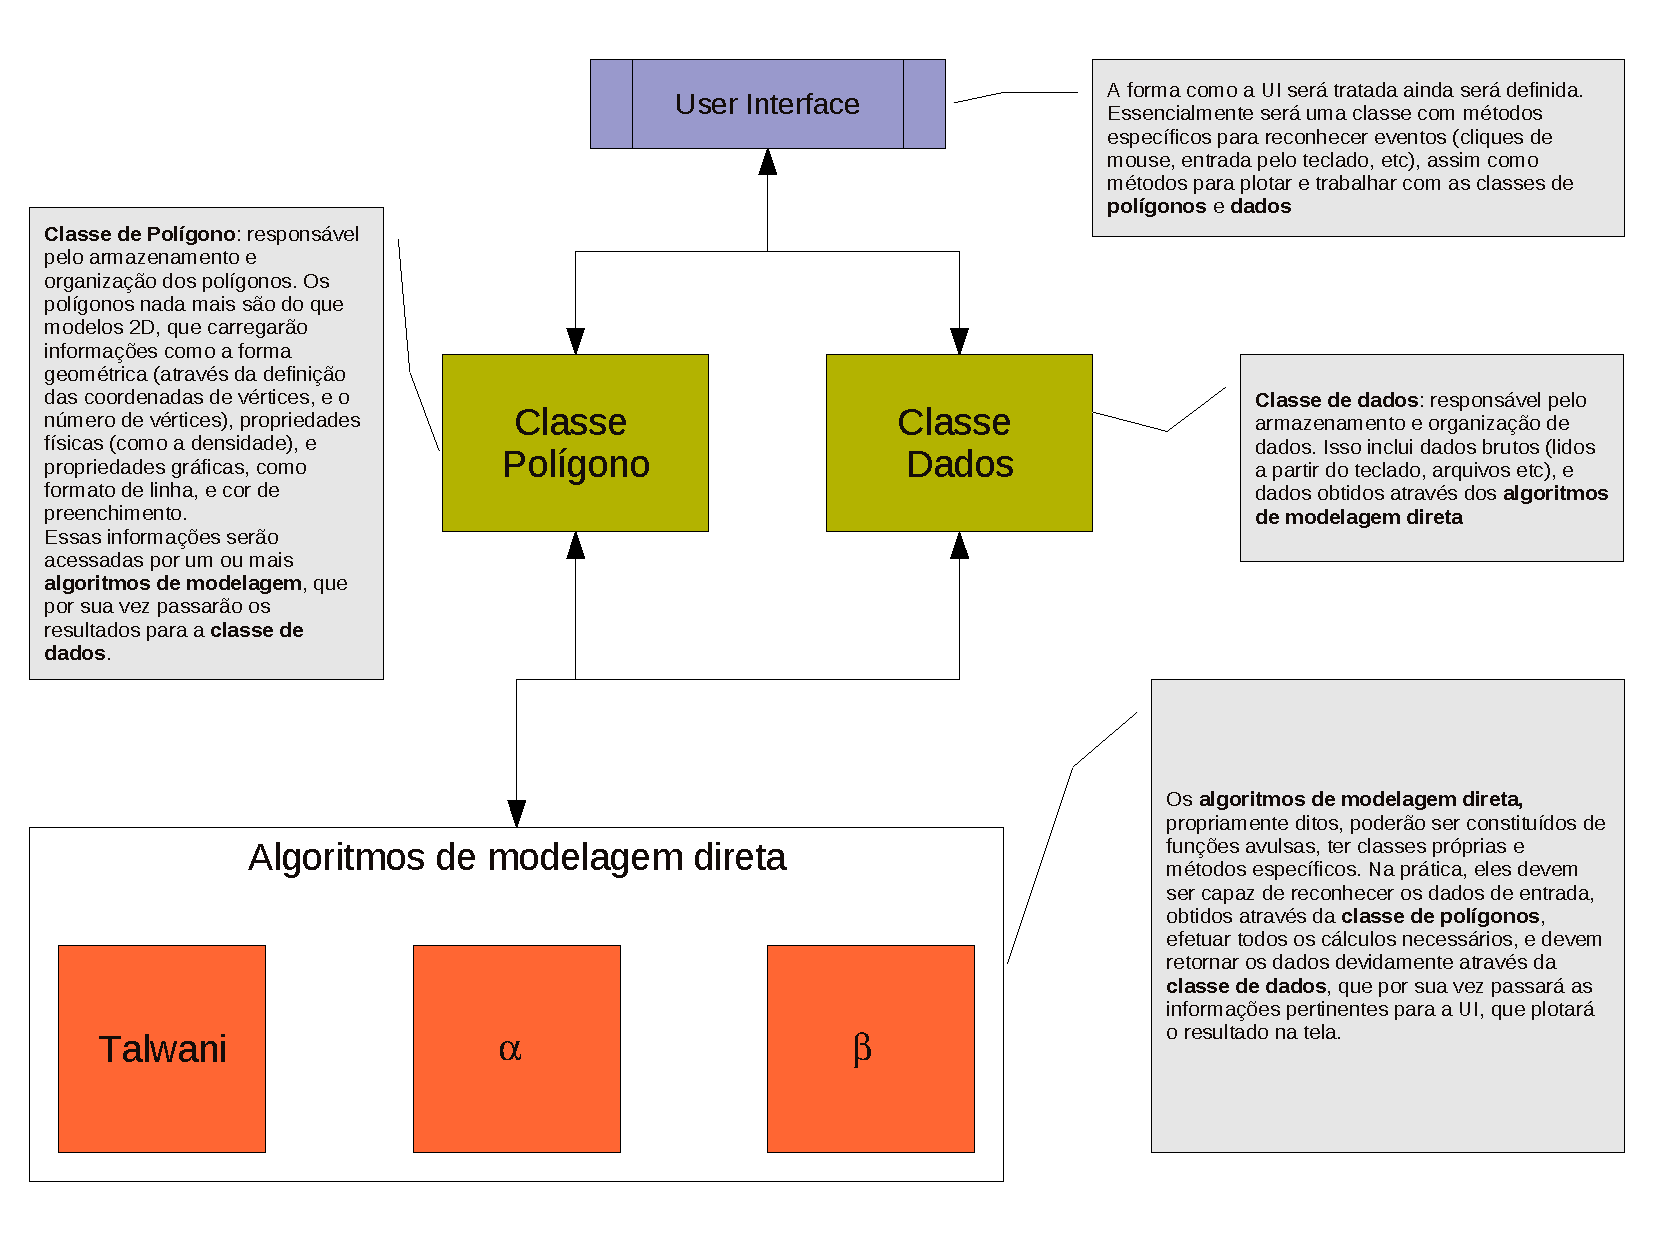
\includegraphics[width=\linewidth]{figs/fluxo-simples.pdf}
    \caption{
        Diagrama de flujo para la primera implementación de un software para el
        modelado gravimétrico de polígonos 2D. Realizado por Leonardo Uieda
        (circa 2009).
    }
    \label{fig:talwani-idea}
\end{figure}

En paralelo, y como proyecto final de su Bachillerato, Leonardo Uieda realiza
una implementación en Python del algoritmo para el cálculo de campos
gravitacionales de tesseroides mediante la \ac{GLQ}.
Luego de reescribirlo en C, este proyecto deriva en el lanzamiento del software
Tesseroids \citep{uieda2016} que ha sido ampliamente utilizado por la comunidad
geocientista.

El éxito de estos proyectos los llevó a aspirar a una idea mucho más
ambiciosa: desarrollar un software de código abierto para modelar el planeta
Tierra de
forma completa.
En ese entonces surge un nombre para el proyecto: \emph{Fatiando a Terra}, que
puede traducirse como \emph{rebanando la Tierra}.

Durante su Master en Geofisica en el Observatório Nacional, Rio de Janeiro,
Leonardo comienza el desarrollo de Fatiando a Terra, transformándolo en el hogar
de las implementaciones que realiza a lo largo de sus investigaciones, todas
mediante el lenguaje Python.
Entre ellas podemos encontrar: modelados directos con diferentes geometrías,
continuación ascendente, deconvolución de Euler, fuentes equivalentes, hasta un
incipiente \emph{framework} de inversión y algunas implementaciones de
tomografías sísmicas simples.

En los años posteriores, cuando la mayoría de los gestores del proyecto se
encontraban cursando sus Doctorados, Fatiando a Terra comienza a cobrar mayor
forma.
Leonardo y Vanderei deciden utilizar el \emph{framework} de inversión para dar
un curso sobre inversiones geofísicas en la Universidade de São Paulo.
Fatiando adquiere su propio dominio
(\href{https://www.fatiando.org}{fatiando.org}) y su primera página web,
alojada en un servidor casero por José Caparica Jr\footnote{%
    Más adelante se utilizarán los servicios de
    \href{https://readthedocs.org/}{Read The Docs} para alojar el sitio web,
    que más tarde se reemplazarían por GitHub Pages.
}.
Además se elige distribuirlo bajo la licencia
\href{https://opensource.org/licenses/BSD-3-Clause}{BSD 3-clause}.
En 2013, el proyecto es presentado en una charla en SciPy 2013
\citep{uieda2013}.

En los años posteriores el proyecto comienza a cobrar mayor reconocimiento.
Empieza a ser utilizado en publicaciones científicas
\citep[][entre otros]{%
    uieda2012,
    carlos2014,
    oliveira2015,
    hidalgogato2015,
    carlos2016,
    reis2016,
    uieda2017,
    hidalgogato2017,
    siqueira2017%
},
% fill in more papers if you know about some others
dictado de clases
(Tópicos de inversão em
geofísica\footnote{%
    \url{https://www.leouieda.com/teaching/inversao-iag-2012.html}
    y \url{https://www.leouieda.com/teaching/inversao-unb-2014.html}
},
\citet{uieda2014},
Geofísica 1: Gravimetria e magnetometria\footnote{%
    \url{https://www.leouieda.com/teaching/geofisica1.html}
},
Geofísica 2: Sismologia e sísmica\footnote{%
    \url{https://www.leouieda.com/teaching/geofisica2.html}
})
y en trabajos finales de grado y posgrado
\citep{carlos2013, sales2014, soler2015, uieda2016b, melo2020}.
Además comienza a atraer la atención de la comunidad internacional, recibiendo
colaboraciones de investigadores y desarrolladores de diferentes partes del
mundo.
La utilización de fatiando por otros investigadores e investigadoras deriva
a su vez en un ciclo de retroalimentación: quienes comienzan siendo usuarios
realizan colaboraciones.
De esta forma fatiando comienza a alojar implementaciones de métodos
novedosos recientemente publicados \citep{uieda2012b, oliveira2013}.

Mi primea contribución al proyecto consistió en una implementación del promedio
radial del espectro de frecuencias de grillas de gravedad
o magnetismo\footnote{%
    \url{https://github.com/fatiando/fatiando/pull/303}
}.
Desde entonces comencé a involucrarme cada vez más en el proyecto, lo que me
permitió adquirir mayores conocimientos en el uso de controladores de
versiones, flujos de trabajo para el desarrollo colaborativo, creación de
funciones de \emph{testing}, buenas prácticas para el diseño de algoritmos y la
importancia de mantener la documentación actualizada.

La última versión del paquete fatiando es la v0.5, lanzada en Noviembre de
2016.
Si bien ese paquete en particular se encuentra obsoleto y no recibe mayor
mantenimiento, esto no significa que la vida de el proyecto haya finalizado en
ese entonces.

A partir de 2018 el proyecto tomó una nueva dirección.
El panorama de software de código abierto para Geofísica había cambiado mucho
desde los inicios de Fatiando a Terra: la cantidad de nuevos paquetes diseñados
para atacar diversos problemas de las geociencias había aumentado
considerablemente
\citep{cockett2015, ruecker2017, varga2019, obspy2019}.
Dentro de este nuevo ecosistema, fatiando no poseía un objetivo claro.
Esto no solo hacía difícil que potenciales usuarios y usuarias identifiquen el
propósito del proyecto, sino que también constituía una base de código difícil
de mantener.
Por otro lado, para ese entonces fatiando había sido el hogar de
implementaciones de métodos clásicos de la geofísica, métodos muy novedosos
(orientados principalmente a la investigación científica), así como de código
\emph{juguete} diseñado para ser utilizado en clases para fines didácticos
pero sin las capacidades para atacar problemas reales.
Sumado a esto, la versión de Python 2.7 llegaba pronto a su final de vida, lo
que hacía necesario adaptar fatiando al nuevo Python 3.

Estas razones ponían en evidencia la necesidad de establecer objetivos claros
para el proyecto, así como también repensar su diseño y sustentabilidad
a futuro.
Por esto se tomó la decisión de dividir el proyecto en varios paquetes que
posean objetivos claros y concisos.
Esto permitiría no sólo una fácil adopción por parte de usuarios y usuarias,
sino también que otros proyectos los utilicen como dependencias en caso de
desearlo.
Además, manteniendo los campos de acción de cada paquete aislados del resto,
se facilitaría el desarrollo a futuro: los colaboradores no necesitan
familiarizarse con el proyecto completo, sino solo con algunas de sus partes.
Por otro lado, la decisión de reescribir gran parte del código se presentó como
una oportunidad para pensar mejores diseños del software ya existente y de
implementar mejores
prácticas para el desarrollo de software, estableciendo estándares de calidad
más altos.


\section{Paquetes de software}

Actualmente Fatiando a Terra está compuesto por cuatro paquetes de software
destinados a ofrecer soluciones a diversas problemáticas en geociencias, así
como también a otras áreas de la ciencia:

\begin{description}
    \item[\emph{Verde}]{%
        Procesado y grillado de datos espaciales
    }
    \item[\emph{Boule}]{%
        Elipsoides de referencia para aplicaciones geodésicas y geofísicas
    }
    \item[\emph{Harmonica}]{%
        Procesado, modelado directo e inverso de datos gravimétricos
        y magnéticos
    }
    \item[\emph{Pooch}]{%
        Descargar y almacenar datos científicos de la web de forma sencilla
    }
\end{description}

\subsection{Verde}

\emph{Verde} ofrece herramientas para procesar datos espaciales (tales como
muestras geofísicas obtenidas en el campo, mediciones de batimetría, etc)
e interpolarlos sobre grillas regulares.

La mayoría de los muestreos de datos espaciales se componen por datos
irregularmente distribuidos sobre la zona de estudio:
puntos dispersos, trayectos irregulares o líneas casi rectas.
Sin embargo, muchas metodologías de procesado e interpretación requieren que
los datos se sitúen sobre puntos pertenecientes a una grilla regular.
Este problema suele resolverse mediante la interpolación de los datos
originales sobre una grilla regular, proceso que se conoce como
\emph{grillado}.

Dentro de los algoritmos de grillado existe una categoría que se conoce como
\emph{interpolaciones con funciones de base radial} (\emph{radial basis
function interpolation} en inglés). Un ejemplo de un algoritmo que entra en
esta categoría son las \emph{splines} biharmónicas.
Estos métodos asumen que podemos representar los datos observados por una
combinación lineal de funciones de Green, es decir:

\begin{equation}
    d_i = \sum_{j=1}^M c_j G(\mathbf{p}_i, \mathbf{q}_j),
\end{equation}

\noindent donde $d_i$ y es el dato $i$-ésimo, $\mathbf{p}_i$ es la ubicación de
ese mismo punto, $c_j$ es un coeficiente escalar, $G$ es una función de Green y
$\mathbf{q}_j$ es la ubicación del punto que define la función de Green en el
término $j$-ésimo.
El proceso de interpolación consiste en ajustar los valores de los
coeficientes $c_j$ mediante mínimos cuadrados de forma tal que se recuperen los
datos observados, y luego utilizarlos para predecir valores sobre los puntos de
la grilla:

\begin{equation}
    d(\mathbf{p}) = \sum_{j=1}^M c_j G(\mathbf{p}, \mathbf{q}_j),
\end{equation}

\noindent donde $\mathbf{p}$ es la ubicación de cualquier punto de la grilla.

Dentro de \emph{Verde} hallamos implementaciones de algoritmos de interpolación
de este tipo siguiendo un diseño similar
a los modelos de aprendizaje automático de \emph{scikit-learn}
\citep{sklearn2011}. Esto permite que quienes estén familiarizados con la
aplicación de métodos de aprendizaje automático en Python puedan fácilmente
entender cómo utilizar la \ac{API} de \emph{Verde}.
Entre los algoritmos de interpolación que se encuentran implementados están las
\emph{splines} biharmónicas, así como métodos más complejos como la
interpolación de vectores 2D con funciones de Green \citep{sandwell2016}.

Como hemos mencionado anteriormente, los interpoladores presentes en
\emph{Verde} han sido implementados mediante clases que reproducen un
comportamiento similar a las clases de \emph{scikit-learn}.
Los interpoladores en verde poseen un método \texttt{fit()} que se usa para
ajustar los parámetros $c_j$ mediante mínimos cuadrados partiendo de un
conjunto de datos y sus ubicaciones. Luego podemos hacer uso del método
\texttt{predict()} para predecir valores en cualquier conjunto de puntos,
o bien usando el método \texttt{grid()} podemos predecir sobre una grilla
regular de puntos.

Además, \emph{Verde} cuenta con utilidades para realizar reducciones por
bloque, una clases para determinación de tendencias polinomiales, funciones
para el manejo de coordenadas, y herramientas para realizar validaciones
cruzadas y selección de modelos.

El diseño de \emph{Verde} permite su extensibilidad: todos los interpoladores
heredan su estructura a partir de una clase base denominada
\texttt{verde.BaseClass}, lo cual permite construir nuevos tipos de
interpoladores de manera sencilla, restando que definir únicamente el tipo de
función de Green a utilizar.
Además, debido a la compatibilidad con las librerías científicas de Python, es
posible integrarlo a flujos de trabajos establecidos con gran facilidad.

La versión v1.0.0 de \emph{Verde} ha sido publicada en el Journal of Open
Source Software luego de un proceso abierto de revisión por pares
\citep{verde2018}.
Podemos acceder a la documentación correspondiente a la última versión estable
de la librería en \href{https://www.fatiando.org/verde}{fatiando.org/verde}.


\subsection{Boule}

\emph{Boule} es una librería que nos permite representar elipsoides de
referencia mediante objetos. Además nos ofrece herramientas para calcular los
campos gravitatorios que estos elipsoides generan y para realizar conversiones
de coordenadas.

Como hemos visto en la sección~\ref{sec:gravedad-terrestre}, un elipsoide de
referencia puede definirse mediante los semiejes mayor $a$ y menor $b$, su masa
total $M$ y su velocidad angular $\omega$.
De forma alternativa pero equivalente, es posible definirlo mediante los
siguientes parámetros:

\begin{itemize}
    \item el semieje mayor $a$,
    \item el achatamiento $f = (a - b) / a$,
    \item la constante gravitacional geocéntrica $GM$ (donde $M$ es la masa
        del elipsoide y $G$ la constante de gravitación universal),
    \item y la velocidad angular $\omega$.
\end{itemize}

Las funcionalidades principales de \emph{Boule} vienen dadas dentro de la clase
\texttt{Ellipsoids}, la cual nos permite definir cualquier elipsoide de
referencia a partir de los parámetros mencionados.
A modo de ejemplo, uno podría definir el elipsoide WGS84 como se muestra en le
Código~\ref{lst:boule-wgs84}.
Sin embargo, \emph{Boule} ya ofrece algunos de los elipsoides de referencia más
ampliamente usados en geodesia y geofísica, tales como el WGS84
(\texttt{boule.WGS84}), el GRS80: Geodetic Reference System
(\texttt{boule.GRS80}) e incluso un elipsoide de referencia para el planeta
Marte definido según los parámetros disponibles en \citet{ardalan2009}
(\texttt{boule.MARS}).

\lstinputlisting[
    float,
    language=Python,
    caption={Ejemplo de definición de elipsoide de referencia con \emph{Boule}},
    label=lst:boule-wgs84
]{chapters/fatiando-examples/boule-wgs84.py}

A su vez, la clase \texttt{Ellipsoids} posee una serie de propiedades que se
calculan a partir de los parámetros que definen cada elipsoide, entre ellos: el
semieje menor $b$, la primera y segunda excentricidad, la excentricidad lineal,
el radio medio del elipsoide (medido desde un sistema geocéntrico), el módulo
del vector aceleración de la gravedad sobre cualquier punto en el ecuador o en
sus polos.
Además, la misma clase ofrece un conjunto de métodos útiles para realizar
cálculos acerca de los campos gravitatorios que genera el elipsoide
y conversión de unidades.
El método \texttt{geocentric\_radius()} nos permite calcular la distancia entre
el centro del elipsoide y cualquier punto de su superficie a partir de su
latitud geodésica o geocéntrica.
Los métodos \texttt{geodetic\_to\_spherical()}
y \texttt{spherical\_to\_geodetic()} nos permiten convertir coordenadas
geodésicas en esféricas geocéntricas o viceversa siguiendo las ecuaciones de
\citet{vermeille2002}.
El método \texttt{normal\_gravity()} implementa la \emph{fórmula cerrada} de
\citet{li2001a} para calcular el módulo de la aceleración de la gravedad
generada por el elipsoide en cualquier punto dado por sus coordenadas
geodésicas.

Si bien \emph{Boule} es una librería que se encuentra en un estado funcional
y puede ser utilizada en investigaciones científicas al día de la fecha, aún no
ha alcanzado su primera versión estable.
Es posible que aún sea necesario realizar modificaciones sobre su diseño en los
planes de incorporar otros tipos de elipsoides, como las esferas o elipsoides
triaxiales.
A pesar de ello, podemos acceder a la documentación correspondiente a la última
versión en \href{https://www.fatiando.org/boule}{fatiando.org/boule}.


\subsection{Harmonica}

\emph{Harmonica} fue creada con la intención de ser el nuevo hogar de aquellas
implementaciones de métodos de procesado y modelado de datos gravimétricos
y magnéticos.
Además, surgió como oportunidad de rediseñar algunas de estas implementaciones
con el objetivo de facilitar su utilización, extensibilidad y mantenimiento
a futuro.

Una de las principales herramientas que ofrece \emph{Harmonica} son las
funciones de modelado directo para distintas geometrías y para diferentes
sistemas de coordenadas.
La geometría más sencilla que hallamos son masas puntuales en coordenadas
esféricas geocéntricas o en coordenadas Cartesianas, implementando las
ecuaciones~\ref{eq:potencial-masa-puntual} y \ref{eq:gz-particula}.
Podemos calculas los campos gravitacionales producidos por masas puntuales
mediante la función \texttt{point\_mass\_gravity()}.
También podemos calcular los campos gravitacionales de prismas rectangulares
mediante el método de \citet{nagy2000} con las correcciones de
\citet{fukushima2020} descriptas en la sección~\ref{sec:prismas-rectangulares},
haciendo uso de la función \texttt{prism\_gravtiy()}.
\emph{Harmonica} también cuenta con una implementación en Python de los
algoritmos de discretización adaptativa y \ac{GLQ} para calcular los campos
gravitacionales de tesseroides con densidad constante, a los cuales podemos
acceder mediante la función \texttt{tesseroid\_gravity()}.
El Código~\ref{lst:harmonica-point-mass} ejemplifica como podemos utilizar la
función \texttt{point\_mass\_gravity()} para calcular la aceleración de la
gravedad producida por dos masas puntuales dadas en coordenadas Cartesianas.

\lstinputlisting[
    float,
    language=Python,
    caption={%
        Ejemplo de cálculo de aceleración de la gravedad producida por dos
        masas puntuales dadas en coordenadas Cartesianas mediante
        \emph{Harmonica}.
    },
    label=lst:harmonica-point-mass
]{chapters/fatiando-examples/harmonica-point-mass.py}

La mayoría de los métodos de modelado directo involucran cómputos moderadamente
complejos, los cuales puede conllevar a un alto costo computacional,
especialmente a la hora de modelar grandes cantidades de geometrías sobre
muchos puntos de observación.
Escribir estas funciones en Python puro resultaría en implementaciones que no
harían un uso eficiente de los recursos computacionales debido a la misma
naturaleza del interprete de Python.
Es por ello que una de las alternativas más viables es recurrir a código
precompilado (escribiendo las implementaciones en lenguajes como C o FORTRAN
y luego añadir \emph{wrappers} de Python) o bien a compilaciones en tiempo de
ejecución.
En los orígenes de de \emph{Harmonica}, hemos optado por realizar nuestras
implementaciones mediante Numba \citep{numba2015}: un compilador de Python de
alto desempeño.
Numba se encarga de precompilar el código que implementa cada uno de estos
algoritmos al momento de ejecutar las funciones por primera vez, utilizando en
adelante los binarios ya compilados.
Mediante este método no solo podemos hacer un uso mucho más eficiente de los
recursos computacionales sino que además podemos habilitar sencillamente la
paralelización de nuestros algoritmos, distribuyendo la tarea en los
núcleos disponibles del procesador donde se está ejecutando.
Además, dada la naturaleza de Numba, no es necesario que distribuyamos los
binarios de \emph{Harmonica} para cada plataforma o sistema operativo: Numba se
encarga de la precompilación durante el tiempo de ejecución.
De esta manera, se simplifica mucho la tarea de distribuir e instalar
\emph{Harmonica} en cualquier tipo de plataforma.
Las decisiones de diseño han permitido que los métodos de \texttt{EQLHarmonic}
reutilicen muchas de las funciones centrales del modelado directo de masas
puntuales, permitiendo no solo un ahorro en cantidad de código, sino también el
reciclado de las oportunidades que estas proveen mediante el compilador Numba,
como paralelizar la construcción de la matriz Jacobiana.

Otra de las capacidades que presenta esta librería es la de realizar cálculos
a partir de los algoritmos de fuentes equivalentes.
La clase \texttt{EQLHarmonic} contiene una implementación del método de fuentes
equivalentes que utiliza fuentes puntuales y la inversa de la distancia como
función de Green (tal y como se describe en la
sección~\ref{sec:equivalent-sources-technique}).
El ajuste de los coeficientes de las fuentes se realiza mediante un algoritmo
de mínimos cuadrados amortiguados, haciendo uso del parámetro de
\emph{amortiguamiento} adimensional introducido en la
sección~\ref{sec:eql_inversion}.
\texttt{EQLHarmonic} permite ajustar fuentes equivalentes dadas en coordenadas
Cartesianas, mientras que \texttt{EQLHarmonicSpherical} nos permite aplicar la
misma metodología pero definiendo las fuentes puntuales y los puntos de
observación en coordenadas esféricas geocéntricas.
Estas clases heredan muchos de los métodos y atributos de la clase
\texttt{BaseGridder} de \emph{Verde}, haciendo que su utilización sea a su vez
muy similar a la que encontramos en los métodos de aprendizaje automático de
scikit-learn \citep{sklearn2011}.

\emph{Harmonica} ofrece además algunas otras funcionalidades de procesado de
datos gravimétricos: aplicación de la corrección de Bouguer utilizando una
aproximación de placa infinita, cálculo de profundidad de raíces según un
modelo isostático de Airy, la capacidad de leer archivos \texttt{.gdf}
provistos por el servicio
ICGEM\footnote{\url{http://icgem.gfz-potsdam.de/home}}, creación de muestras
sintéticas aéreas o sobre terreno a partir de muestras reales.

Si bien \emph{Harmonica} es una librería que se encuentra en un estado funcional
y puede ser utilizada en investigaciones científicas al día de la fecha, aún no
ha alcanzado su primera versión estable.
A pesar de ello, podemos acceder a la documentación correspondiente a la última
versión en \href{https://www.fatiando.org/harmonica}{fatiando.org/harmonica}.

% Planes a futuro:

% incluir gradient-boosted eqls y variable density tesseroids

% derivadas espaciales de grillas (verticales con FFT)

% Euler deconvolution

% inversion: nuevo framework de inversion

\subsection{Pooch}

\emph{Pooch} nos ofrece herramientas para descargar datos científicos alojados
en Internet, almacenarlos localmente y comprobar sus sumas de verificación,
entre otras características.

Muchas de las librerías de software científico hacen uso de datos de muestra
para ejemplificar su funcionamiento en las secciones de la documentación que se
conocen como \emph{Galería de ejemplos}.
Usualmente estos datos de muestra se incluyen dentro de los repositorios donde
se aloja el mismo código fuente de la librería, sin embargo estos archivos de
datos no son empaquetados para su distribución con el objetivo de reducir el
tamaño de las futuras instalaciones.
En cambio, los datos de muestra suelen ser descargados al ser necesarios
mediante código implementado dentro de cada una de estas librerías, haciendo
uso de paquetes de Python para descargar archivos mediante protocolo HTTP por
ejemplo.
\emph{Pooch} surge como una solución a este problema transversal a muchas
librerías del ecosistema científico de Python.

\lstinputlisting[
    float,
    language=Python,
    caption={%
        Ejemplo de descarga de archivos con \emph{Pooch} mediante la
        clase \texttt{pooch.Pooch}. Este código es a modo de ejemplificación
        y no está escrito para ser ejecutado.
    },
    label=lst:pooch-registry
]{chapters/fatiando-examples/pooch-registry.py}


\emph{Pooch} permite gestionar un \emph{registro} en el cual podemos listar las
direcciones de cada uno de los archivos que queremos ofrecer para su descarga,
junto con el \emph{hash} de una suma de verificación. Al solicitar alguno
o algunos de estos archivos, \emph{Pooch} se encarga de descargarlos de su
correspondiente localización, almacenarlos en un \emph{caché} local y realizar
una suma de verificación con el objetivo de certificar la integridad de los
mismos.
La descarga de los archivos se lleva a cabo únicamente si no existe tal archivo
en el \emph{caché} local.
En el Código~\ref{lst:pooch-registry} podemos visualizar cómo es posible
utilizar la función \texttt{pooch.create()} para inicializar una instancia de
la clase \texttt{pooch.Pooch} especificando el directorio donde se descargarán
los archivos, la dirección base donde se encuentran alojados los archivos de
interés, y el \emph{registro} donde especificamos el nombre de los archivos
y sus \emph{hashes} de las sumas de verificación.
Luego podemos solicitar la descarga de uno de los archivos mediante el método
\texttt{fetch()}, el cual devuelve la ruta al archivo descargado y almacenado
localmente.

\emph{Pooch} no sólo nos permite descargar archivos desde el protocolo HTTPS,
sino también desde FTP y SFTP con autenticación.
Incluso es posible descargar archivos almacenados en repositorios de acceso
abierto como Zenodo\footnote{\url{https://zenodo.org/}}
o figshare\footnote{\url{https://figshare.com}} únicamente mediante el
\ac{DOI}.
A su vez, también soporta diferentes tipos de suma de verificación, como
SHA256, MD5, XXH128, entre otras.
Además ofrece la posibilidad de realizar post-procesados luego de la descarga
de los archivos, como por ejemplo descomprimir archivos \texttt{.zip},
\texttt{.tar}, \texttt{.gzip}, \texttt{.xz}, etc.

El paquete presenta ciertas cualidades que lo hacen un excelente candidato para
ser utilizado por librerías de terceros.
En primer lugar, es posible configurarlo para que se adapte a diferentes
necesidades en pocas líneas con una sintaxis sencilla.
En segundo lugar, es un paquete puramente escrito en Python con dependencias
mínimas.
Y por último, presenta un alto grado de extensibilidad: es posible definir
funciones propias para otro tipos de descargas (mediante otros protocolos, por
ejemplo) o bien para realizar post-procesados. Estas funciones personalizadas
puede acoplarse fácilmente al \emph{framework} de \emph{Pooch}, permitiendo
utilizar su misma sintaxis y sus capacidades de descarga, almacenamiento
y comprobación de sumas de verificación, incluso en aplicaciones particulares.

La versión v0.7.1 de \emph{Pooch} fue publicada en el Journal of Open Source
Software luego de una revisión abierta por pares \citep{pooch2020}.

\lstinputlisting[
    float,
    language=Python,
    caption={%
        Ejemplo de descarga de archivos con \emph{Pooch} mediante la
        función \texttt{pooch.retrieve()}.
    },
    label=lst:pooch-retrieve
]{chapters/fatiando-examples/pooch-retrieve.py}

Hasta entonces la principal audiencia de \emph{Pooch} consistía en otros
desarrolladores de software que deseaban una forma sencilla de distribuir datos
de muestra a sus usuarios.
Sin embargo, en los meses subsiguientes se presentó la oportunidad de incluir
otro tipo de audiencia al paquete: usuarios finales que deseaban descargar
pocos archivos por única vez.
Esto se materializó con la creación de la función \texttt{pooch.retrieve()} que
permite acceder a las mismas funcionalidades de \emph{Pooch}, pero sin la
necesidad de predefinir una instancia de \texttt{pooch.Pooch} y con una
interfaz más sencilla.
El Código~\ref{lst:pooch-retrieve} ejemplifica cómo podemos utilizar la función
\texttt{pooch.retrieve()} para descargar un archivo, almacenarlo localmente
y comprobar su suma de verificación en una única ejecución.
La función devuelve la ruta al archivo descargado y almacenado localmente.

Actualmente \emph{Pooch} es utilizado por varias librerías del ambiente
científico, entre ellas: MetPy \citep{metpy}, icepack \citep{icepack}, MOABB
\citep{moabb}, MNE-Python \citep{mnepython}, junto a otras librerías de
Fatiando como \emph{Harmonica} y \emph{Verde}.
Además, otras librerías de Python con aplicaciones más amplias han incluido
a \emph{Pooch} dentro de sus dependencias, por ejemplo Xarray
\citep{xarray2017} y scikit-image \citep{skimage}.

La documentación correspondiente a la última versión estable de \emph{Pooch}
puede hallarse en \href{https://www.fatiando.org/pooch}{fatiando.org/pooch}.


\section{Desarrollo y mejores prácticas}
\label{sec:best-practices}

Desde sus orígenes, el proyecto ha sido desarrollado siguiendo las mejores
prácticas que se encontraban en conocimiento de sus desarrolladores.
Es por esta razón que a lo largo de sus años de vida se hayan incorporado cada
vez mayor cantidad o mejores herramientas para desempeñar estas mejores
prácticas, a medida que los desarrolladores adquirían mayores conocimientos.

Todo desarrollo de Fatiando a Terra se realiza mediante un software de
controlador de versiones, y a excepción de algunos momentos en la concepción
del proyecto, utilizamos \texttt{git}\footnote{\url{https://git-scm.com}} como
controlador de versiones distribuido
y GitHub\footnote{\url{https://www.github.com}} como servidor de repositorios.

Gracias a \texttt{git}, cada librería posee una \emph{rama} principal de
desarrollo donde se provee del código fuente que será utilizado por los
usuarios y usuarias finales.
El flujo de desarrollo de cada una de las librerías del proyecto se basa en los
\emph{Issues} y \emph{Pull Requests} que ofrece GitHub.
En cada \emph{Issue} ponemos en evidencia la existencia de un problema
existente en el código de la \emph{rama} principal, exponemos una nueva idea
a implementar a futuro o solicitamos una nueva capacidad o comportamiento del
código existente.
Los \emph{Issues} representan un canal de comunicación entre toda la comunidad,
incluyendo usuarios, desarrolladores y contribuidores.

Cada vez que alguien desea colaborar con alguna modificación o una nueva
implementación, esta persona escribe su código en una nueva \emph{rama} que
se desprende de la principal y abre un \emph{Pull Request}, es decir, una
solicitud a los mantenedores de incluir ese nuevo código en la rama principal.
Dentro de los \emph{Pull Requests} otros colaboradores pueden realizar una
revisión del código, sugerir cambios y discutir alternativas, de forma tal que
la propuesta inicial alcance el estado necesario para poder ser incorporada
al código fuente de la librería.
Los requisitos para que un nuevo código sea aceptado no son estrictos, sin
embargo se busca alcanzar un determinado estándar de calidad siguiendo un
conjunto de mejores prácticas.
Las revisiones de código no tienen como objetivo determinar si una cierta
contribución debe ser aceptada o rechazada, sino que se toman como punto de
partida para aplicar las modificaciones necesarias hasta alcanzar dicho
estándar de calidad.

Muchas de las mejores prácticas que aplicamos a lo largo del proyecto pueden
hallarse en \citet{wilson2014,wilson2017}, sin embargo presentamos
a continuación una descripción detallada de las más importantes.

\subsection{Estilo de escritura}

El lenguaje Python admite estilos de escritura muy variados, priorizando que el
código sea legible a poseer una sintaxis muy estricta.
Sin embargo, a la hora de mantener una base de código entre muchos
desarrolladores, es recomendable establecer un estilo de escritura común.
Dentro del proyecto hemos decidido seguir los lineamientos establecidos en
PEP8 (siglas en inglés de \emph{Python Enhancement Proposals}, propuestas de
mejoras de Python)\footnote{\url{https://www.python.org/dev/peps/pep-0008/}}.
Dentro de estos lineamientos se establecen recomendaciones acerca del tipo de
\emph{indentación} (sangrado) que se debe utilizar; la cantidad máxima de
caracteres por línea; la cantidad de líneas vacías antes y después de la
definición de funciones, clases y métodos; la forma en que se deben nombrar las
variables, las funciones y las clases; entre muchas otras.

Con el objetivo de facilitar la tarea de adecuar cualquier nuevo código a estas
reglas, tanto para quien lo escribe como para quien lo revisa, hemos
normalizado el uso del auto-formateador
Black\footnote{\url{https://black.readthedocs.io/en/stable/}}, el cual
modifica automáticamente cualquier código sintácticamente correcto para seguir
muchos de los lineamientos establecidos en PEP8.
De esta forma, los contribuidores pueden utilizar el estilo de escritura que
les sea más cómodo y luego correr Black para poder adecuarlo al estilo que
adoptamos en Fatiando.

Sin embargo, Black no es capaz de aplicar algunas de las recomendaciones
establecidas en PEP8, especialmente las que tienen que ver con el nombre de las
variables, el modo de uso de operadores lógicos, entre otras.
Para este tipo de situaciones hacemos uso de otro software que permite detectar
este tipo de errores además de muchas otras recomendaciones para mejorar la
escritura de nuestro código: pylint\footnote{\url{https://pylint.org/}}.
pylint no solo identifica violaciones a PEP8, sino que además realiza un
análisis más profundo del código: desde detectar variables definidas pero no
utilizadas, módulos importados innecesariamente, definiciones de funciones
extremadamente largas o con muchos argumentos entre muchas otras.
Dentro del proyecto utilizamos pylint para identificar este tipo de errores más
difíciles de detectar, sin embargo establecemos un criterio más flexible:
permitimos ignorar alguna de sus recomendaciones si lo consideramos
conveniente.

\subsection{Documentación}

% Flujo de trabajo en Github.

% Code review.

% Code style. Black. Lint

% Documentación.

% Testeo.

% CI.

% Ejemplos.

% Filosofía UNIX?

% Releases y backward compatibility?

% Pypi y conda-forge?


\section{Comunidad}

Codigo de conducta

Instructivos para contribuir

Reuniones periodicas

Discusiones abiertas en issues/PRs

Interacción con otros proyectos?


\section{Adopción en la comunidad científica}

Publicaciones científicas relacionadas.

Tutoriales en Transform2020 y Transform 21 charla para la GSH

Visitas a la página web


\section{Planes a futuro}

Stable release of every package

Mayor interoperabilidad con el resto de paquetes geofísicos (SimPEG, pyGIMLi, etc)

Implementar esféras en boule (luna, mercurio).
Implementar elipsoides traixiales en boule.
Unificar las clases de elipsoides para todo tipo.


\bibliographystyle{apalike-doi}
\bibliography{references}
\addcontentsline{toc}{chapter}{Bibliografía}

\end{document}
